\chapter{Fundamentos}

\section{Introdução}

% Neste capítulo, busca-se apresentar uma revisão abrangente dos conceitos fundamentais e das principais abordagens na literatura relacionada à classificação de textos curtos. A compreensão desses conceitos é importante para contextualizar e fundamentar as discussões e análises nos capítulos subsequentes.

% A organização do capítulo é a seguinte: inicia-se com uma seção sobre os conceitos fundamentais, onde são definidos e explicados os principais conceitos e terminologias relacionados à classificação de textos curtos. Avança-se, então, para a revisão da literatura, abrangendo áreas como a evolução histórica do tema, abordagens convencionais e técnicas de aprendizado de máquina aplicadas à classificação de textos curtos. Será realizada uma análise crítica das técnicas existentes, destacando suas limitações, lacunas e controvérsias na literatura, e a relevância da pesquisa atual em relação aos trabalhos anteriores.

% Ao final do capítulo, conclui-se os principais pontos discutidos, estabelecendo uma base sólida para os capítulos subsequentes. Esta estrutura visa uma compreensão do estado da arte no campo da classificação de textos curtos e a identificação de oportunidades para pesquisa futura e desenvolvimento de novas técnicas.


Neste capítulo, apresenta-se uma revisão dos conceitos básicos e das principais abordagens na literatura relacionada à classificação de textos curtos. Esses conceitos são importantes para contextualizar as discussões e análises nos capítulos subsequentes.

O capítulo está organizado da seguinte forma: inicialmente, são definidos e explicados os conceitos e terminologias principais. Em seguida, realiza-se uma revisão da literatura, cobrindo a evolução histórica do tema, abordagens convencionais e técnicas de aprendizado de máquina aplicadas à classificação de textos curtos. Além disso, é feita uma análise crítica das técnicas existentes, destacando suas limitações e a relevância da pesquisa atual.

Ao final do capítulo, resume-se os principais pontos discutidos, estabelecendo uma base para os capítulos subsequentes. Esta estrutura busca proporcionar uma visão geral do estado da arte na classificação de textos curtos e identificar oportunidades para futuras pesquisas e desenvolvimento de novas técnicas.

\section{Classificação de Texto Curto}

\subsection{Definição}

A Classificação de texto consiste em atribuir uma classe ou categoria pré-definida a um conjunto de texto. É uma tarefa comum em processamento de linguagem natural e é utilizada para organizar, estruturar e categorizar grandes quantidades de dados \cite{kowsari2019text} .

Os algoritmos de classificação de texto recebem como entrada um conjunto de texto e produzem uma classe. A classe é escolhida a partir de um conjunto pré-definido de categorias ou rótulos. 
Formalmente, de acordo com \cite{aggarwal2012survey}, um problema de classificação envolve um conjunto de instâncias $D = {X_1,...,X_n}$, onde cada instância pertence a uma das $k$ classes indexadas por ${1,2,...,k}$. Aqui, $X_i$ é um exemplo, como uma descrição de produto, e $n$ é o número de instâncias. Na Figura \ref{fig:produtos_categorias}, é apresentada a associação entre as descrições dos itens e suas respectivas categorias, onde se observa $n=3$ itens distintos relacionados às suas classes ($k=2$).

\begin{figure}[htbp]
    \centering
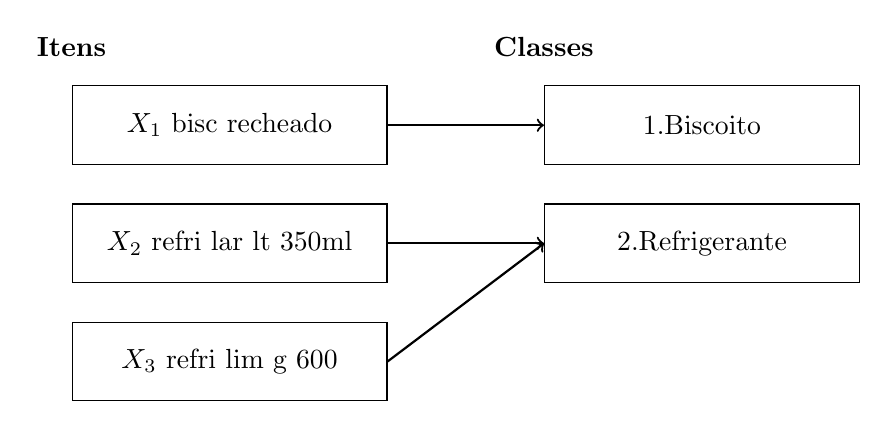
\begin{tikzpicture}[
    box/.style={draw, rectangle, minimum width=4cm, minimum height=1cm, anchor=west},
    title/.style={font=\bfseries},
    arrow/.style={->, thick}
]

% Titles
\node[title] (itemdesc) at (0,0) {Itens};
\node[title] (classes) at (6,0) {Classes};

% Left column items
\node[box] (x1) at (0,-1) {$X_1$ bisc recheado};
\node[box] (x2) at (0,-2.5) {$X_2$ refri lar lt 350ml};
\node[box] (x3) at (0,-4) {$X_3$ refri lim g 600};

% Right column categories
\node[box] (c1) at (6,-1) {1.Biscoito};
\node[box] (c2) at (6,-2.5) {2.Refrigerante};

% Arrows
\draw[arrow] (x1.east) -- (c1.west);
\draw[arrow] (x2.east) -- (c2.west);
\draw[arrow] (x3.east) -- (c2.west);

\end{tikzpicture}

\caption{Associação de produtos e suas categorias}
    \label{fig:produtos_categorias}
\end{figure}

Um conjunto de treinamento é usado para construir um modelo de classificação, que é utilizado para prever a classe de uma nova instância desconhecida. Este problema pode ser considerado difícil quando a classe é explicitamente determinada ou suave quando são atribuídas probabilidades. A classificação de texto requer a conversão de texto em dados numéricos, o que pode ser alcançado por meio de técnicas de processamento de linguagem natural, mostrados em seção posterior.

\subsubsection{Texto Curto}

Texto curto é definido, extraído de \cite{alsmadi2019review} como um texto de até 200 caracteres.

\subsection{Dificuldades}

Apesar de possuir as mesmas definições, um texto curto, até 200 caracteres \cite{alsmadi2019review}, acrescenta algumas dificuldades.  Na Tabela \ref{tab:desafios_textos_curtos}, são apresentados os principais desafios na classificação de textos curtos conforme \cite{alsmadi2019review} e \cite{song2014short}:

\begin{table}[h!]
\centering
\begin{tabular}{l|p{4cm}|p{8cm}}
\hline
\textbf{Nº} & \centering\textbf{Desafio} & \textbf{Breve descrição} \\
\hline
1 & \centering Contexto limitado & Textos curtos geralmente têm pouco contexto ou informações básicas. \\
\hline
2 & \centering Vocabulário limitado & Textos curtos podem ter um número limitado de palavras ou atributos, o que pode dificultar a extração de informações significativas para classificação. \\
\hline
3 & \centering Ruído & Textos curtos podem conter erros ortográficos, abreviações ou outras formas de ruído. \\
\hline
4 & \centering Estilo informal ou não estruturado & Textos curtos, como tweets ou resenhas de produtos, geralmente têm um estilo informal ou não estruturado. \\
\hline
5 & \centering Alto grau de variabilidade & Textos curtos podem variar significativamente em termos de comprimento, conteúdo e linguagem, o que pode dificultar a construção de modelos que generalizem bem para diferentes tipos de textos curtos. \\
\hline
6 & \centering Esparsidade & Textos curtos podem ter um alto grau de esparsidade, o que significa que eles contêm um grande número de atributos de valor zero ou ausentes. \\
\hline
7 & \centering Dados de treinamento limitados & Textos curtos podem ser mais difíceis de classificar com precisão devido à quantidade limitada de dados de treinamento disponíveis, especialmente para aplicações especializadas. \\
\hline
8 & \centering Ambiguidade & Textos curtos são mais propensos a conter informações ambíguas ou incompletas, o que pode dificultar que um classificador determine a classe correta. \\
\hline
\end{tabular}
\caption{Desafios na classificação de textos curtos}
\label{tab:desafios_textos_curtos}
\end{table}


\subsection{Aplicações}

A tabela \ref{tab:exemplos} extraída do texto \cite{bhavani2021review} apresenta exemplos de aplicações para a classificação de textos curtos. Além disso, destaca-se como o aprendizado de máquina e as técnicas de processamento de linguagem natural (PNL) têm evoluído ao longo dos anos, e como elas são aplicadas para resolver problemas de classificação de textos curtos \cite{alsmadi2019review}.  % Discussão expandida com referência adicionada

\begin{table}[h]
\centering
\caption{Exemplos de aplicações para a classificação de textos curtos}
\label{tab:exemplos}
\begin{tabular}{p{6cm}|p{8cm}}
\hline
\textbf{Aplicação} & \textbf{Descrição} \\
\hline
Análise de mídia social & Textos curtos, como tweets ou postagens do Facebook, são comuns em plataformas de mídia social e podem ser classificados de acordo com várias categorias, como sentimento, tópico ou relevância.\\
\hline
Análise de feedback do cliente & Textos curtos, como avaliações de clientes ou respostas a pesquisas, podem ser classificados de acordo com várias categorias, como satisfação, recursos do produto ou classificação geral.\\
\hline
Recuperação de informações & Textos curtos, como consultas de pesquisa ou títulos de documentos, podem ser classificados de acordo com sua relevância para um tópico ou conjunto de palavras-chave específicos.\\
\hline
Análise de sentimento & Textos curtos, como avaliações online ou postagens nas redes sociais, podem ser classificados de acordo com o sentimento que expressam (positivo, negativo ou neutro).\\
\hline
Detecção de spam & Textos curtos, como linhas de assunto de e-mail ou mensagens de texto, podem ser classificados como spam ou não spam.\\
\hline
Modelagem de tópicos & Textos curtos, como títulos de notícias ou artigos científicos, podem ser classificados de acordo com os tópicos que abordam.\\
\hline
\end{tabular}
\end{table}

\subsubsection{Processo de Classificação}

O processo de classificação de textos curtos envolve as mesmas etapas de uma classificação de texto normal, porém \cite{song2014short} sugere uma etapa de enriquecimento de atributos.  As etapas são, adaptado de \cite{kowsari2019text}, \cite{alsmadi2019review} e \cite{aggarwal2018review}:

\textbf{Coleta de dados}: A primeira etapa na classificação de textos curtos é reunir um conjunto de dados de textos curtos que precisam ser classificados. Isso pode ser feito por meio de raspagem de dados da web, coleta manual ou usando conjuntos de dados disponíveis publicamente.

\textbf{Pré-processamento de dados}: Uma vez que os textos tenham sido coletados, realiza-se o pré-processamento para remover qualquer ruído ou informação irrelevante. Isso envolve segmentação de palavras, remoção de palavras frequentes, radicalização e outras técnicas.

\textbf{Tokenização}: Realizada a preparação dos dados o documento, texto ou descrição deve ser quebrado em pedaços menores(tokens).

\textbf{Extração de atributo}: Em seguida, é preciso extrair atributos dos textos pré-processados para representar o conteúdo dos textos de forma numérica que possa ser usada por um classificador. Técnicas comuns de extração de recursos incluem sacola de palavras (\textit{Bag of Words - BoW}), Frequência de Termos (TF), Frequência de termos ponderada pelo inverso da frequência de termos (TF-IDF) e representações de palavras em espaços semânticos (\textit{word embeddings)}.

\textbf{Seleção de modelo e avaliação}: Uma vez que os atributos tenham sido extraídos, um classificador pode ser treinado com os dados e avaliado para determinar sua precisão. Diferentes classificadores podem ser comparados usando técnicas dividindo o conjunto em treino e teste ou realizando validação cruzada.  Várias métricas de avaliação podem ser usadas para medir o desempenho do classificador.

\textbf{Implantação do modelo}: Se o desempenho do classificador for satisfatório, ele pode ser implantado para classificar novos textos conforme forem surgindo.

Nas seções subsequentes é detalhado as fases de pré-processamento, tokenização e extração de atributos.

\subsection{Pré-processamento}\label{subsec:preprocessamento}

A literatura sugere que as técnicas de pré-processamento têm um impacto significativo na classificação de textos, \cite{naseem2021survey}. Podem influenciar significativamente o desempenho dos classificadores. Imperfeições nos dados, tais como ruídos introduzidos por elementos não estruturados ou linguagem informal, podem degradar a eficácia dos modelos de classificação.

\cite{naseem2021survey} realizou uma análise detalhada de 12 técnicas distintas de pré-processamento e relatou que, enquanto algumas técnicas resultam em melhorias, outras podem impactar negativamente o desempenho. Mais ainda, foi identificado que a ordem na qual essas técnicas são aplicadas é um fator relevante, pois sequências inadequadas podem levar à perda de informações.

Esta descoberta ressalta a importância de uma abordagem sistemática e bem pensada no pré-processamento de textos curtos, visando otimizar os resultados da classificação e minimizar a perda de informações essenciais.

A sequencia abaixo enumera as 12 técnicas do artigo \cite{naseem2021survey} e acrescenta uma técnica relevante para o contexto de descrição de produtos.

\begin{enumerate}
    \item \textbf{Remoção de Ruído (URLs, Hashtags e Menções de Usuários):} Técnica que envolve a eliminação de elementos como URLs, hashtags e menções de usuários, considerados ruídos em dados de texto, especialmente em tweets.
    \begin{itemize}
        \item \textbf{Exemplo (Antes):} "Confira em www.google.com \#Tecnologia @usuario"
        \item \textbf{Exemplo (Depois):} "Confira em ."
    \end{itemize}

    \item \textbf{Substituição de Emoticons e Emojis:} Esta técnica substitui emoticons e emojis por seus respectivos significados em palavras, ajudando na captura de sentimentos e opiniões expressos através desses símbolos.
    \begin{itemize}
        \item \textbf{Exemplo (Antes):} Eu estou tão feliz \emoji{smile}
        \item \textbf{Exemplo (Depois):} Eu estou tão feliz smile
    \end{itemize}

    \item \textbf{Substituição de Abreviações e Gírias:} Envolve a conversão de abreviações e gírias em seus significados completos em palavras. 
    \begin{itemize}
        \item \textbf{Exemplo (Antes):} Refri Coca Cola \textbf{LT} 350ml
        \item \textbf{Exemplo (Depois):} Refri Coca Cola \textbf{lata} 350ml
    \end{itemize}

    \item \textbf{Tratamento de Caracteres Alongados:} Lida com palavras em que caracteres são intencionalmente repetidos para ênfase (por exemplo, "loooovvveee"), convertendo-as para suas formas base para evitar que sejam tratadas como palavras diferentes ou fora do vocabulário.
    \begin{itemize}
        \item \textbf{Exemplo (Antes):} Eu amoooooo muiiiiiiito esse lugar!
        \item \textbf{Exemplo (Depois):} Eu amo muito esse lugar!
    \end{itemize}

    \item \textbf{Correção de Ortografia e Gramática:} A correção de erros ortográficos e gramaticais ajuda a reduzir variações da mesma palavra escrita de maneira diferente, contribuindo para a normalização do texto.
    \begin{itemize}
        \item \textbf{Exemplo (Texto Original):} "Eu vou commer piza hooje."
        \item \textbf{Exemplo (Após Correção):} "Eu vou \textcolor{red}{comer} \textcolor{green}{pizza} \textcolor{red}{hoje}."
    \end{itemize}

    \item \textbf{Expansão de Contrações:} Contrações e palavras abreviadas são expandidas para suas formas completas, padronizando o texto para processamento mais fácil por máquinas.
    \begin{itemize}
        \item \textbf{Exemplo (Antes):} "I don't do this."
        \item \textbf{Exemplo (Depois):} "I do not do this."
    \end{itemize}
    Para o contexto de descrição de produtos, existe por exemplo o símbolo de polegadas ", que pode ser expandido para a palavra polegadas.

    \item \textbf{Remoção de Pontuação:} Inclui a remoção de pontuações que, embora expressem sentimentos e emoções, podem não ser úteis para a classificação automática de textos curtos.
    \begin{itemize}
        \item \textbf{Exemplo (Antes):} "Eu estou tão feliz!!!"
        \item \textbf{Exemplo (Depois):} "Eu estou tão feliz"
    \end{itemize}
    Para o contexto de descrição de produtos, quando a pontuação representa abreviação é possível removê-lo sem perda de informação como por exemplo em "bisc.recheado".

    \item \textbf{Remoção de Números:} Trata-se da eliminação de numerais presentes nos textos, embora se deva ter cuidado para não perder informações importantes nesse processo.
    \begin{itemize}
        \item \textbf{Exemplo (Antes):} "Havia 5 pássaros no jardim."
        \item \textbf{Exemplo (Depois):} "Havia pássaros no jardim."
    \end{itemize}
    Para o contexto de descrição de produtos, a remoção de número implica em retirada de informação relevante, pois as apresentações dos produtos são características de categorias, por exemplo, enquanto bebidas possuem padrões de volumetria como 350, 600 e 1, categorias como feijão possuem números como 500, 1, 2 e 5.  

    \item \textbf{Conversão para Minúsculas (Folding to Lower-casing):} Consiste em converter todas as letras maiúsculas para minúsculas para evitar variações da mesma palavra determinadas pelo uso de maiúsculas e minúsculas.
    \begin{itemize}
        \item \textbf{Exemplo (Antes):} "Este é um Exemplo."
        \item \textbf{Exemplo (Depois):} "este é um exemplo."
    \end{itemize}

    \item \textbf{Remoção de Palavras Comuns (Stop-words):} Envolve a eliminação de palavras de alta frequência que contribuem pouco para o significado semântico do texto.  As palavras frequentes são palavras comuns que não têm muito significado, como "o", "e" ou "mas". Remover palavras frequentes reduz a dimensionalidade dos dados e melhora a eficiência do classificador.
    \begin{itemize}
        \item \textbf{Exemplo (Antes):} "O livro é muito bom."
        \item \textbf{Exemplo (Depois):} "livro bom."
    \end{itemize}

    \item \textbf{Lematização:} Processo que transforma palavras em suas formas base, utilizando conhecimento lexical em vez de simplesmente cortar as inflexões das palavras.
    \begin{itemize}
        \item \textbf{Exemplo (Antes):} \textbf{Corri} para a floresta e \textbf{vi} muitos \textbf{cervos}.
        \item \textbf{Exemplo (Depois):} \textbf{Correr} para a floresta e \textbf{ver} muitos \textbf{cervo}."
    \end{itemize}
    \item \textbf{Segmentação de Palavras:} A segmentação de palavras é o processo de separar as frases/conteúdos/palavras usadas em uma hashtag, ou seja, \#algumtópico é segmentado em duas palavras: algum + tópico. 
    \begin{itemize}
        \item \textbf{Exemplo (Antes):} "\#TendênciasDeTecnologia estão em alta hoje!"
        \item \textbf{Exemplo (Depois):} "Tendências De Tecnologia estão em alta hoje!"
    \end{itemize}
    \item \textbf{Remoção de Acentuação}:  Esta técnica não é incluída no artigo de \cite{naseem2021survey}, mas para a língua portuguesa, tem-se uma quantidade significativa de palavras com acento.  A remoção de acentuação objetiva normalizar as palavras retirando seus acentos e reduzindo a variabilide de escrita.  Por exemplo, a palavra feijão possui em muitas descrições apenas a escrita feijao que representa a mesma palavra acentuada.
    \begin{itemize}
        \item \textbf{Exemplo (Antes):} "\textbf{Tendências} de tecnologia \textbf{estão} em alta!"
        \item \textbf{Exemplo (Depois):} "\textbf{Tendencias} de tecnologia \textbf{estao} em alta!"
    \end{itemize}      
\end{enumerate}

A Tabela \ref{table:preprocessamento} apresenta as técnicas de pré-processamento aplicadas na classificação de descrições de produtos, juntamente com uma justificativa para a aplicação ou não aplicação de cada técnica. Foram aplicadas apenas as técnicas de conversão para minúsculas e remoção de acentuação. A conversão para minúsculas é importante para padronizar a escrita, evitando variações desnecessárias. A remoção de acentuação normaliza palavras acentuadas e não acentuadas, reduzindo a variabilidade. Outras técnicas, como substituição de abreviações e gírias, correção de ortografia e gramática, expansão de contrações, remoção de pontuação, segmentação de palavras e remoção de números, não foram aplicadas porque, conforme \cite{naseem2021survey}, contribuem pouco para a melhoria no contexto de descrições de produtos e podem resultar na perda de informações relevantes.

\begin{table}[h]
\centering
\begin{tabular}{c|p{5cm}|c}
\hline
Número & Técnica & Aplicação (Sim/Não) \\
\hline
1 & Remoção de Ruído (URLs, Hashtags e Menções de Usuários) & Não \\
\hline
2 & Substituição de Emoticons e Emojis & Não \\
\hline
3 & Substituição de Abreviações e Gírias & Não \\
\hline
4 & Tratamento de Caracteres Alongados & Não \\
\hline
5 & Correção de Ortografia e Gramática & Não \\
\hline
6 & Expansão de Contrações & Não \\
\hline
7 & Remoção de Pontuação & Não \\
\hline
8 & Remoção de Números & Não \\
\hline
9 & Conversão para Minúsculas (Folding to Lower-casing) & Sim \\
\hline
10 & Remoção de Palavras Comuns (Stop-words) & Não \\
\hline
11 & Lematização & Não \\
\hline
12 & Segmentação de Palavras & Não \\
\hline
13 & Remoção de Acentuação & Sim \\
\hline
\end{tabular}
\caption{Técnicas de pré-processamento aplicadas na classificação de descrição de produtos}
\label{table:preprocessamento}
\end{table}

\subsection{Tokenização}\label{subsec:tokenizacao}
  Tokenização é o processo de dividir um texto em palavras ou tokens individuais. Isso é geralmente feito usando uma combinação de espaços em branco, pontuação e caracteres especiais como delimitadores.
  
\begin{itemize}
   \item \textbf{n-grama}: Outra técnica utilizada refere-se uma forma de segmentação chamada n-grama.  Um n-grama é uma sequência contígua de n itens de um determinado conjunto de texto. Os n-gramas são frequentemente usados em processamento de linguagem natural e recuperação de informação como uma maneira de extrair informações adicionais do texto.
Os n-gramas podem ser extraídos de qualquer conjunto de texto e o valor de n pode ser ajustado para capturar diferentes quantidades de contexto. Por exemplo, os 1-grama (também conhecidos como unigramas) capturam palavras individuais, enquanto os 3-gramas (também conhecidos como trigramas) capturam grupos de três palavras consecutivas.
    \item \textbf{Skip-grama}: Um skip-grama é uma variante do modelo n-grama que é utilizada para capturar dependências de longo alcance. Assim como os n-gramas tradicionais, os skip-gramas são sequências de palavras contíguas de um determinado conjunto de texto. No entanto, ao contrário dos n-gramas tradicionais, os skip-gramas permitem "pular" algumas palavras no texto, em vez de exigir que todas as palavras da sequência sejam consecutivas.
\end{itemize}

A tabela \ref{tab:exemplopreprocessamento} demonstra uma sequencia de aplicação para a descrição  "Arroz tio joão 1.kg".

\begin{table}[!htp]
\centering

\begin{tabular}{l|l}
\hline
Técnica                                       & Resultado                                      \\ 
\hline
Descrição Original       & Arroz tio joão 1.kg                            \\
Remoção de pontuação     & Arroz tio joão 1 kg                            \\
Remoção de acentuação    & Arroz tio joao 1 kg                            \\
Conversão para minúscula & arroz tio joao 1 kg                            \\
unigramas                & \{arroz, tio, joao, 1, kg\}                    \\
bigramas                 & \{(arroz, tio), (tio, joao), (joao,1),(1,kg)\} \\ 
1-skip-2-grama          & \{(arroz, joao), (tio,1), (joao,kg) \} \\
\hline
\end{tabular}
\caption{Aplicação de técnicas de pré-processamento e tokenização sobre o texto \textit{Arroz tio joão 1.kg}}
\label{tab:exemplopreprocessamento}
\end{table}

\subsection{Representação Numérica e Extração de Atributos}\label{subsec:representacaonumerica}

A representação numérica dos textos é a parte essencial para sua utilização com algoritmos de aprendizado de máquina.  Após a aplicação das técnicas de pré-processamento e tokenização, gera-se um conjunto conhecido como vocabulário, que consiste de todos os types (tokens distintos) de todos os documentos ou descrições.  A partir deste conjunto, inicia-se as fases de extração, seleção, ponderação e embutimento dos seus elementos, não sendo necessariamento obrigatórias nem exclusivas.  

A extração de atributos é o processo de extrair características relevantes de um conjunto de dados, que podem então ser usadas para treinar um modelo de aprendizado de máquina. No contexto da classificação de texto, a extração de características envolve selecionar as palavras ou combinações de palavras mais relevantes e informativas do texto para serem usadas como entrada para o modelo.  Os modelos utilizados para classificação requerem entradas numéricas, desta forma é necessário converter os textos para números.

Um processo que é similar consiste na tarefa de seleção de características, conforme delineado por \cite{du2019feature}, engloba um processo de identificação, avaliação e seleção das características mais relevantes para uma questão de pesquisa específica. Esta tarefa pode melhorar a precisão dos modelos de classificação, contribuindo para a redução da complexidade do modelo e ampliando a interpretabilidade dos resultados.  No estudo de \cite{du2019feature} as características são categorizadas em cinco grupos principais: semântica, sentimento, legibilidade, estrutura e sintaxe.  
As características semânticas enfocam no conteúdo e no significado implícito das palavras nas avaliações, enquanto as de sentimento examinam as emoções expressas pelos autores. A legibilidade avalia a facilidade de leitura e compreensão da avaliação, a estrutura relaciona-se à organização e ao formato do texto, e as características de sintaxe investigam o uso de diferentes classes gramaticais na escrita. 
Conforme observado por \cite{du2019feature}, os resultados do estudo indicam que as categorias de semântica e sentimento são mais eficazes na previsão da utilidade das avaliações em comparação com as categorias de legibilidade, estrutura e sintaxe, mostrando a importância do conteúdo e emoção expressos nas avaliações para a percepção dos usuários.

Para a tarefa de classificação de texto contida neste trabalho, não há interesse no sentimento, desta forma, destaca-se a importância das características \textbf{semânticas}.  Estas características são extraídas diretamente das palavras contidas no texto.

A forma mais utilizada pelos pesquisadores é a representação de cada palavra como um vetor. A partir deste é possível gerar uma combinação de ponderação ou embutimentos.  As próximas seções apresentam as técnicas Sacola de Palavras (Bag of Words - BoW), Frequência de Termos(Term Frequency - TF) e Frequencia de Termos ponderada pela Frequencia Inversa de Documentos(Term Frequency Inverse Document Frequency-TFIDF).

\subsection{Modelo Sacola de Palavras (Bag of Words-BoW): Frequência de Termos e Modelo Booleano(Binário)}

Uma técnica amplamente adotada para a representação numérica de documentos é o modelo de sacola de palavras ou /textbf{Bag of Words (BoW)}. Conforme descrito por \cite{deng2019feature}, neste modelo, um documento é representado por uma lista de pares \((s_j, f_j)\), onde \(s_j\) representa um termo e \(f_j\) denota a frequência desse termo no documento \(d_i\). Este modelo simplifica a representação textual ao abstrair a ordem e a estrutura gramatical das palavras, focando apenas na presença e na frequência dos termos.  Já para \cite{zhang2010understanding}, envolve atribuir um valor numérico a cada palavra em uma descrição e representar a descrição como um vetor que indica a presença ou ausência de cada palavra, com um valor de 1 indicando a presença da palavra e 0 indicando sua ausência.  Este último é conhecido como modelo booleano ou binário.

\subsection{Exemplo de Sacola de Palavras}
\label{sec:exemplo-sacola-de-palavras}
Este exemplo demonstra a aplicação dessa técnica nas descrições: "Arroz tio joão 1 kg", "ARROZ FUMACENCE PARB 1KG", "FEIJAO CARIOCA 1KG AZULAO", "Feij 1 Kg Preto Caldão".  

As etapas envolvidas são:

\begin{enumerate}
    \item Remoção de acentos e conversão para minúsculas:
    \begin{itemize}
        \item "Arroz tio joão 1 kg" → "arroz tio joao 1 kg"
        \item "ARROZ FUMACENCE PARB 1KG" → "arroz fumacence parb 1kg"
        \item "FEIJAO CARIOCA 1KG AZULAO" → "feijao carioca 1kg azulao"
        \item "Feij 1 Kg Preto Caldão" → "feij 1 kg preto caldao"
    \end{itemize}
    \item Divisão das descrições em tokens (palavras) no formato unigrama:
    \begin{itemize}
        \item Descrição 1: ["arroz", "tio", "joao", "1", "kg"]
        \item Descrição 2: ["arroz", "fumacence", "parb", "1kg"]
        \item Descrição 3: ["feijao", "carioca", "1kg", "azulao"]
        \item Descrição 4: ["feij", "1", "kg", "preto", "caldao"]
    \end{itemize}
    \item Criação de um vocabulário com tokens únicos:
    \begin{itemize}
        \item Tokens Distintos: ["arroz", "tio", "joao", "1", "kg", "fumacence", "parb", "1kg", "feijao", "carioca", "azulao", "feij", "preto", "caldao"]
    \end{itemize}
    \item Contagem da frequência de cada token nas descrições, tabela \ref{tab:bow}.
\end{enumerate}

\begin{table}
\begin{tabular}{c|l|c|c|c|c|c}
\hline
Número do Type & Type & [1] & [2] & [3] & [4] & [5] \\
\hline
1 & 1 & 0 & 1 & 0 & 0 & 1 \\
2 & 1kg & 0 & 0 & 1 & 1 & 0 \\
3 & arroz & 1 & 1 & 1 & 0 & 0 \\
4 & azulao & 0 & 0 & 0 & 1 & 0 \\
5 & caldao & 0 & 0 & 0 & 0 & 1 \\
6 & carioca & 0 & 0 & 0 & 1 & 0 \\
7 & feij & 0 & 0 & 0 & 0 & 1 \\
8 & feijao & 0 & 0 & 0 & 1 & 0 \\
9 & fumacence & 0 & 0 & 1 & 0 & 0 \\
10 & joao & 0 & 1 & 0 & 0 & 0 \\
11 & kg & 0 & 1 & 0 & 0 & 1 \\
12 & parb & 0 & 0 & 1 & 0 & 0 \\
13 & preto & 0 & 0 & 0 & 0 & 1 \\
14 & tio & 0 & 1 & 0 & 0 & 0 \\
\hline
\end{tabular}
\caption{Vocabulário, representação de uma palavra como vetor em [1] e representação das demais descrições em [2],[3],[4] e [5] para "Arroz tio joão 1 kg", "ARROZ FUMACENCE PARB 1KG", "FEIJAO CARIOCA 1KG AZULAO", "Feij 1 Kg Preto Caldão" respectivamente}
\label{tab:bow}
\end{table}

A representação de cada palavra é um vetor com um 1 na posição correspondente à posição da palavra no vocabulário e 0s em todas as outras posições. Por exemplo, "arroz" seria representado por \{1,0,0,0,0,0,0,0,0,0,0,0,0,0\}, conforme exemplo na tabela \ref{tab:bow}. Para representar uma descrição, 
 esta é pré-processada e tokenizada e, em seguida, cada token é convertido em sua representação vetorial. Finalmente, esses vetores são somados, o que equivale a uma contagem de palavras. Por exemplo, a descrição 'Feijao Preto Caldao Preto 1kg' é representado por \{0,0,0,0,0,0,0,0,1,1,0,0,0,2,1\}.  

A tabela \ref{tab:bow} pode ser visualizada de maneira transposta, com cada documento ou descrição nas linhas e o vocabulário nas colunas. Esta representação é chamada de matriz termo-documento D, com \( d_{ij} \) representando a frequência do termo \( j \) no documento \( i \). As dimensões da matriz \( |D| \times |V| \) são definidas pelo número de documentos \( |D| \) e o número de termos no vocabulário \( |V| \).

 Devido a alta dimensionalidade do vocabulário uma seleção de atributos é sugerida, \cite{mironczuk2018recent}.  \cite{deng2019feature} em seu artigo descreve os processos de filtragem e extração de características com o objetivo de identificar atributos que sejam representativos e informativos para as categorias em foco. Esta abordagem garante que o modelo de classificação minimize a redundância e a esparsidade dos dados, e também melhore sua capacidade de generalização e precisão preditiva. 
 
Para efetuar essa seleção, \cite{deng2019feature}, técnicas como ganho de informação, TF-IDF (Term Frequency-Inverse Document Frequency) e teste \(\chi^2\) são utilizadas para identificar os atributos mais significativos, também chamadas de modelos de filtro.  Além da seleção de atributos, técnicas de projeção como Análise Semântica Latente (LSA) e Análise de Componentes Principais (PCA) são empregadas para reduzir a dimensionalidade.  Estas técnicas não são objetos de estudo deste trabalho.

\subsection{O Modelo TF-IDF}

O Term Frequency-Inverse Document Frequency (TF-IDF) é uma técnica de ponderação de termos amplamente utilizada em sistemas de recuperação de informações e classificação de texto\cite{baeza2013recuperaccao}. O modelo equilibra a necessidade de identificar termos relevantes em documentos individuais (frequência do termo - TF) e a raridade desses termos em uma coleção de documentos (frequência inversa do documento - IDF).

A frequência do termo (TF) indica quantas vezes um termo aparece em um documento específico, proporcionando uma medida da importância do termo nesse documento. No entanto, para evitar que termos comuns em muitos documentos sejam considerados excessivamente importantes, o modelo TF-IDF utiliza o componente IDF. A frequência inversa do documento (IDF) é calculada como o logaritmo do número total de documentos na coleção dividido pela frequência do documento do termo, ou seja, o número de documentos em que o termo aparece. Matematicamente, o peso TF-IDF de um termo em um documento é expresso como:

\begin{equation}
    w_{ij} = tf_{ij} \times \log\left(\frac{|D|}{df_i}\right)
\end{equation}

onde \( w_{ij} \) é o peso do termo \( i \) no documento \( j \), \( tf_{ij} \) é a frequência do termo \( i \) no documento \( j \), \( |D| \) é o número total de documentos na coleção, e \( df_i \) é a frequência do documento do termo \( i \).

Além disso, \cite{salton1988term} enfatiza a importância da normalização desses pesos para evitar distorções. A normalização é realizada dividindo o peso TF-IDF de um termo em um documento pela raiz quadrada da soma dos pesos TF-IDF desse documento em todos os termos. A fórmula de normalização é dada por:

\begin{equation}
    w'_{ij} = \frac{w_{ij}}{|w_{.j}|}
\end{equation}

onde

\begin{equation}
    |w_{.j}| = \sqrt{\sum_{i}{w_{ij}^2}}
\end{equation}

representa a norma do pesos $w_{ij}$ para o documento \( j \), calculada como a raiz quadrada da soma dos quadrados dos pesos TF-IDF de todos os termos \( i \) no documento \( j \).

Esta normalização assegura que os termos são ponderados não apenas pela sua frequência e raridade, mas também pela sua importância relativa em toda a coleção de documentos, proporcionando uma avaliação mais precisa e equilibrada da relevância de cada termo.

\subsection{Exemplo de Aplicação do TF-IDF}
\label{sec:exemplo-tfidf}
Este exemplo aplica a técnica TF-IDF nas descrições anteriormente tratadas na seção "Sacola de Palavras" (veja a Seção \ref{sec:exemplo-sacola-de-palavras}). O TF-IDF é calculado com base na frequência do termo em cada descrição e na frequência inversa do documento para cada termo.

As etapas envolvidas são:

\begin{enumerate}
    \item Utilização das descrições e do vocabulário já processados conforme descrito na Seção \ref{sec:exemplo-sacola-de-palavras}.
    \item Cálculo dos pesos IDF, \( w_{ij} \) e \( w'_{ij} \) para cada token nas descrições.
\end{enumerate}

A Tabela \ref{tab:tfidf} exemplifica a implementação do método TF-IDF, partindo das descrições abordadas na seção ``Sacola de Palavras''. Nesta tabela, observa-se a interação entre a frequência de um termo em uma descrição específica ($f_{ij}$) e sua frequência inversa em todo o conjunto de documentos (IDF), resultando no peso TF-IDF ($wij$) de cada termo. É possível observar que palavras como ``arroz'', ``1'', ``kg'' e ``1kg'', que aparecem em mais de uma descrição, têm sua importância diminuída pelo componente IDF, refletindo a perda de força destes termos comuns. A normalização aplicada, resultando no valor $w'_{ij}$, ajusta o peso TF-IDF baseado na norma dos pesos dos termos do documento. No contexto deste trabalho, onde as descrições de produtos são tipicamente curtas, esta normalização não influencia significativamente a análise individual de cada descrição. Portanto, embora a normalização seja um passo relevante, seu impacto é menos pronunciado em análises de descrições curtas, mantendo a eficácia do modelo TF-IDF em contextos de processamento de linguagem natural aplicado a descrições de produtos.

\begin{table}[h]
    \centering
    \scriptsize
    \begin{tabular}{c|l|c|c|c|c|c}
    \hline
    Código & Type & IDF & [1] & [2] & [3] & [4] \\
    \hline
    {} & {} & {} & \( f_{ij} \) | \( wij \) | \( w'ij \) & \( f_{ij} \) | \( wij \) | \( w'ij \) & \( f_{ij} \) | \( wij \) | \( w'ij \) & \( f_{ij} \) | \( wij \) | \( w'ij \) \\
    \hline
    0  & 1         & 0.69 & 1 | 0.69 | 0.30 & 0 | 0.00 | 0.00 & 0 | 0.00 | 0.00 & 1 | 0.69 | 0.27 \\
    1  & 1kg       & 0.69 & 0 | 0.00 | 0.00 & 1 | 0.69 | 0.32 & 1 | 0.69 | 0.28 & 0 | 0.00 | 0.00 \\
    2  & arroz     & 0.69 & 1 | 0.69 | 0.30 & 1 | 0.69 | 0.32 & 0 | 0.00 | 0.00 & 0 | 0.00 | 0.00 \\
    3  & azulao    & 1.39 & 0 | 0.00 | 0.00 & 0 | 0.00 | 0.00 & 1 | 1.39 | 0.55 & 0 | 0.00 | 0.00 \\
    4  & caldao    & 1.39 & 0 | 0.00 | 0.00 & 0 | 0.00 | 0.00 & 0 | 0.00 | 0.00 & 1 | 1.39 | 0.53 \\
    5  & carioca   & 1.39 & 0 | 0.00 | 0.00 & 0 | 0.00 | 0.00 & 1 | 1.39 | 0.55 & 0 | 0.00 | 0.00 \\
    6  & feij      & 1.39 & 0 | 0.00 | 0.00 & 0 | 0.00 | 0.00 & 0 | 0.00 | 0.00 & 1 | 1.39 | 0.53 \\
    7  & feijao    & 1.39 & 0 | 0.00 | 0.00 & 0 | 0.00 | 0.00 & 1 | 1.39 | 0.55 & 0 | 0.00 | 0.00 \\
    8  & fumacence & 1.39 & 0 | 0.00 | 0.00 & 1 | 1.39 | 0.63 & 0 | 0.00 | 0.00 & 0 | 0.00 | 0.00 \\
    9  & joao      & 1.39 & 1 | 1.39 | 0.60 & 0 | 0.00 | 0.00 & 0 | 0.00 | 0.00 & 0 | 0.00 | 0.00 \\
    10 & kg        & 0.69 & 1 | 0.69 | 0.30 & 0 | 0.00 | 0.00 & 0 | 0.00 | 0.00 & 1 | 0.69 | 0.27 \\
    11 & parb      & 1.39 & 0 | 0.00 | 0.00 & 1 | 1.39 | 0.63 & 0 | 0.00 | 0.00 & 0 | 0.00 | 0.00 \\
    12 & preto     & 1.39 & 0 | 0.00 | 0.00 & 0 | 0.00 | 0.00 & 0 | 0.00 | 0.00 & 1 | 1.39 | 0.53 \\
    13 & tio       & 1.39 & 1 | 1.39 | 0.60 & 0 | 0.00 | 0.00 & 0 | 0.00 | 0.00 & 0 | 0.00 | 0.00 \\
    \hline
    $|w_{.j}|$ & & & 2.30 & 2.19 & 2.50 & 2.59 \\
    \hline
    \end{tabular}

    \caption{Análise TF-IDF das descrições "Arroz tio joão 1 kg", "ARROZ FUMACENCE PARB 1KG", "FEIJAO CARIOCA 1KG AZULAO", e "Feij 1 Kg Preto Caldão". A tabela mostra a frequência de termos $(f_{ij})$, o peso TF-IDF $(w_{ij})$ e o peso normalizado TF-IDF $(w'_{ij})$ para cada termo nas descrições.}
    \label{tab:tfidf}
\end{table}

\subsection{Modelos de Projeção - Redução de Dimensionalidade}

A projeção de características é uma parte opcional na classificação de texto, onde algoritmos como Análise de Componentes Principais (PCA), Decomposição de Valor Singular (SVD) e Alocação Latente de Dirichlet (LDA) são frequentemente utilizados. Esses métodos são empregados para reduzir a dimensionalidade dos dados, mantendo ao mesmo tempo as características mais relevantes para a classificação. A PCA é uma técnica estatística que transforma os dados originais em um conjunto de valores de componentes principais linearmente descorrelacionados. A SVD, por outro lado, decompõe uma matriz em três outras matrizes, capturando a essência dos dados. A LDA é um modelo generativo que permite explicar conjuntos de observações por meio de grupos não observados que explicam por que algumas partes dos dados são semelhantes. A utilização dessas técnicas de projeção ajuda a melhorar a eficiência e a precisão dos modelos de classificação de texto, permitindo que eles lidem melhor com a alta dimensionalidade e a complexidade dos dados textuais \cite{mironczuk2018recent}.   Detalha-se a seguir a técnica de Análise Semântica Latente (LSA) devido a sua significativa relevância na literatura.  \cite{pu2006short}.

\subsubsection{Análise Semântica Latente (LSA)}

A Análise Semântica Latente (LSA) é uma técnica para a geração automática de conceitos e análise da coocorrência de termos, útil para a classificação de texto e recuperação de informações \cite{pu2006short}. Baseando-se na decomposição em valores singulares (SVD), a LSA permite a construção de uma matriz de documento reduzida, A, que mantém apenas as informações mais cruciais da matriz de documento original. A representação matemática da LSA é dada por:

\begin{equation}
    A = TSD^T
\end{equation}

Nesta fórmula, T e D são compostos por vetores ortogonais, enquanto S é uma matriz diagonal de valores singulares. Os autovetores com os maiores valores singulares capturam os eixos de maior variação nos dados, permitindo a projeção de cada documento em um espaço de dimensionalidade inferior. Este processo de redução de dimensionalidade permite diminuir o ruído nos dados e evitar o sobreajuste.

A utilização da LSA na classificação de textos (TC) facilita a identificação de padrões e temas subjacentes, que podem não ser direto em análises textuais diretas. Ao focar nas características mais significativas dos documentos através da redução da dimensionalidade, a LSA melhora a eficácia dos algoritmos de classificação e recuperação de informações.

\subsection{Word Embeddings}

Word embeddings(a tradução é incorporação ou embutimento, para fins subsequentes é mantido o original em inglês), é uma abordagem que transforma palavras em vetores de números reais, permitindo que palavras com contextos semelhantes sejam correlacionadas. Embora os primeiros métodos, como one-hot encoding, oferecessem representações básicas, a evolução para técnicas mais avançadas permitiu a captura de relações semânticas e das semelhanças entre as palavras. É seguido aqui a abordagem de \cite{selva2021review}.  Os embeddings são categorizados em três tipos principais: Tradicional, Estático e Contextualizado.  

Os embeddings tradicionais foram apresentados nas seções anteriores.  Cita-se aqui apenas as vantagens e desvantagens.  Essas abordagens têm limitações, como a falta de representação das relações semânticas entre palavras e a necessidade de grande capacidade de memória.  

\subsubsection{Word Embedding Estática}

Os Embeddings Estáticos, como Word2Vec, GloVe e Fast Text, oferecem representações fixas que não variam com o contexto. Eles representam uma evolução em relação a métodos anteriores, fornecendo probabilidades às palavras e mapeando-as em vetores densos. Esses métodos são estáticos no sentido de que mantêm a mesma representação independentemente do contexto. A tabela \ref{tab:wordembstatic}, adaptada de \cite{selva2021review}, apresenta para Word2Vec, GloVe e Fast Text uma breve descrição, vantagens e desvantagens.

\begin{table}[h]
\centering
\scriptsize
\begin{tabular}{l|p{3cm}|p{3cm}|p{3cm}}
\hline
\textbf{Modelo} & \textbf{Descrição} & \textbf{Vantagens} & \textbf{Desvantagens} \\
\hline
Word2Vec & Gera embedding de palavras usando representação densa. & Transforma um corpus não rotulado em dados rotulados mapeando a palavra para um contexto. & Não utiliza informações globais; \\
\hline
GloVe & Modelo baseado em contagem e não supervisionado para gerar vetores de palavras. & Baseia-se em informações de contexto local e estatísticas globais (co-ocorrência de palavras); pode derivar relações semânticas. & Dependente da matriz de co-ocorrência; requer mais memória para armazenamento. \\
\hline
Fast Text & Extensão do Word2Vec que identifica palavras como n-gramas de caracteres. & Fornece representação vetorial eficiente de palavras raras e fragmentos de palavras. & Não adiciona informações contextuais. \\
\hline
\end{tabular}
\caption{Comparação de Modelos de Embedding Estático}
\label{tab:wordembstatic}
\end{table}

\subsubsection{Embedding Contextualizado}

Os Embeddings Contextualizados, como ELMo, GPT-2 e BERT, oferecem representações dinâmicas que variam com base no contexto. Eles são capazes de capturar nuances contextuais e semânticas, oferecendo múltiplos embeddings para uma única palavra. Tais modelos têm demonstrado um bom desempenho em uma variedade de tarefas de NLP.  A tabela \ref{tab:wordembcontext}, retirado de \cite{selva2021review} apresenta para ELMo, GPT-2 e BERT uma breve descrição, vantagens e desvantagens.

\begin{table}[h]
\centering
\scriptsize
\begin{tabular}{l|p{3cm}|p{3cm}|p{3cm}}
\hline
\textbf{Modelo} & \textbf{Descrição} & \textbf{Vantagens} & \textbf{Desvantagens} \\
\hline
ELMo & Embedding context-dependent e baseado em caracteres. & Fornece múltiplos embeddings de palavras para uma única palavra. & Bidirecional superficial, não pode aproveitar contextos à esquerda e à direita simultaneamente. \\
\hline
GPT-2 & Transformer que prediz a próxima palavra observando partes de uma frase. & Pode prever a próxima palavra e oferecer várias possíveis previsões com pontuação de probabilidade. & Requer grande capacidade de computação; pode criar informações falsas, pois é treinado em milhões de sites. \\
\hline
BERT & Sistema bidirecional não supervisionado com um codificador Transformer multicamada. & Aprende as relações contextuais entre palavras ou subpalavras; contém significados sintáticos e semânticos; pode fazer suposições para a palavra em branco. & Limitado a lidar com frases de comprimento mínimo. \\
\hline
\end{tabular}
\caption{Comparação de Modelos de Embedding Contextualizado}
\label{tab:wordembcontext}
\end{table}

\section{Técnicas para Classificação de Texto}

Na parte um é apresentada uma adaptação da teoria de recuperação da informação para a classificação de produtos.
Na seção dois é apresentada as principais técnicas de Machine Learning NB, DT, KNN, SVM, bagging, boosting, RF.
Na seção três as técnicas de redes neurais.

\subsection{Classificação de Texto a partir da Função de Ordenação da Recuperação da Informação}

A recuperação da informação (RI) concentra-se em localizar e prover informações pertinentes em resposta a consultas específicas. Sua aplicação tem sido aplicada em sistemas de busca, como os encontrados na web, e no gerenciamento de grandes repositórios de documentos.

Uma formulação formal da RI foi proposta por \cite{baeza2013recuperaccao}, definindo um modelo de RI como uma quádrupla \([D,Q,\mathcal{F}, R(q_i,d_j)]\), onde:

\begin{enumerate}
    \item \( D \) representa um conjunto de documentos de uma coleção.
    \item \( Q \) compreende as representações das necessidades de informação dos usuários, denominadas consultas.
    \item \( \mathcal{F} \) fornece a estrutura para modelar tanto os documentos quanto as consultas e suas inter-relações, utilizando-se de conjuntos, relações booleanas, vetores e operações de álgebra linear, bem como espaços amostrais e distribuições de probabilidade.
    \item \( R(q_i,d_j) \) é uma função de ranqueamento que atribui um valor real a cada par formado por uma consulta \( q_i \) e um documento \( d_j \), estabelecendo uma ordenação dos documentos em face da consulta \( q_i \).
\end{enumerate}


Como ilustrado na Figura~\ref{fig:ri_model}, o modelo de recuperação de informação recebe um consulta, converte para uma representação numérica e para cada documento aplica uma função de ordenação.

\begin{figure}[ht]
\centering
\begin{tikzpicture}[node distance=2cm, auto]
  % Nodes
  \node (consulta) [draw, rectangle] {consulta};
  \node (qi) [draw, rectangle, right=of consulta] {\(q_i\)};
  \node (documentos) [draw, rectangle, below=1.5cm of consulta] {documentos};
  \node (dj) [draw, rectangle, right=of documentos] {\(d_j\)};
  \node (R) [draw, rectangle, right=2.5cm of qi] {\(R(q_i, d_j)\)};

  % Arrows
  \draw[-{Latex[length=3mm]}] (consulta) -- (qi);
  \draw[-{Latex[length=3mm]}] (documentos) -- (dj);
  \draw[-{Latex[length=3mm]}] (qi) -- (R);
  \draw[-{Latex[length=3mm]}] (dj) -- (R);
\end{tikzpicture}
\caption{Modelo de recuperação de informação representando a interação entre consulta, documentos e a função de ranqueamento.}
\label{fig:ri_model}
\end{figure}

\subsection{Adaptação da Recuperação da Informação para Classificação}

Neste estudo realizou-se uma adaptação da definição tradicional de RI ao contexto de classificação de produtos. O elemento essencial é o conjunto de descrições (ainda não rotulada).  Na sequencia define-se um conjunto de classes.  Aplica-se uma função de mapeamento, tornando um conjunto de descrições de produtos em classes (documentos), comumente executada por intervenção humana.  De forma a retornar para a definição do modelo tradicional de RI.

A RI, no domínio da classificação de produtos, foi reformulada como uma sêxtupla \( ( X, Y, \mathcal{M},Q, R, \mathcal{C} \)), na qual:
\begin{itemize}
    \item \( X \) é um conjunto de representações das descrições dos produtos.
    \item \( Y \) abrange um conjunto de classes previamente definidas.
    \item \( \mathcal{M}: X \to Y \) descreve a função de mapeamento que associa descrições de produtos a suas respectivas classes a priori.
    \item \( Q \) compreende as descrições de produto a classificar.
    \item \( \mathcal{C}: X \to Y \) descreve a função de mapeamento que associa descrições de produtos a suas respectivas classes a posteriori, ou classificador.    
\end{itemize}

Conforme mostrado na Figura~\ref{fig:ri_adapted_model}, a adaptação do modelo de recuperação de informação para a classificação de produtos é ilustrada. Este modelo expande a interação tradicional entre consultas e documentos para incluir uma etapa adicional de mapeamento para classes de produtos.

\begin{figure}[ht]
\centering
\begin{tikzpicture}[node distance=2cm, auto]
  % Nodes
  \node (descriptions) [draw, rectangle] {descrições};
  \node (documentos) [draw, rectangle, right=of descriptions] {documentos};
  \node (dj) [draw, rectangle, right=of documentos] {\(d_j\)};
  \node (consulta) [draw, rectangle, above=1.5cm of documentos] {consulta};
  \node (qi) [draw, rectangle, right=of consulta] {\(q_i\)};
  \node (R) [draw, rectangle, right=of qi] {\(R(q_i, d_j)\)};
  \node (c) [draw, rectangle, right=of R] {\(\mathcal{C}\)};

  % Arrows
  \draw[-{Latex[length=3mm]}] (descriptions) -- (documentos);
  \draw[-{Latex[length=3mm]}] (documentos) -- (dj);
  \draw[-{Latex[length=3mm]}] (consulta) -- (qi);
  \draw[-{Latex[length=3mm]}] (qi) -- (R);
  \draw[-{Latex[length=3mm]}] (dj) -- (R);
  \draw[-{Latex[length=3mm]}] (R) -- (c);
\end{tikzpicture}
\caption{Adaptação do modelo de RI para classificação de produtos, incorporando a etapa de mapeamento para classes.}
\label{fig:ri_adapted_model}
\end{figure}

No modelo tradicional de Recuperação da Informação (RI), o foco principal é na busca e ordenação de documentos em resposta a consultas específicas. Essa abordagem é bem representada pela função \( R(q_i, d_j) \), que avalia a relevância de um documento \( d_j \) em relação a uma consulta \( q_i \). Este modelo é amplamente utilizado em motores de busca e sistemas de gerenciamento de informações, onde a prioridade é encontrar a melhor correspondência possível para as consultas dos usuários dentro de um vasto conjunto de documentos.

Em contraste, a adaptação do modelo de RI para a classificação de produtos se concentra na categorização de descrições de produtos em classes predefinidas. Esta adaptação introduz a função \( \mathcal{C}: X \to Y \), onde \( \mathcal{C} \) é responsável pelo mapeamento da ordenação em sua classe correspondentes.

Diferenças entre os dois modelos incluem:

\begin{itemize}
    \item No modelo tradicional de RI, a ordenação dos documentos é a principal operação, enquanto na adaptação para classificação de produtos, o foco é na posterior categorização das descrições.
    \item A função \( \mathcal{M} \) no modelo adaptado serve como uma etapa de treinamento para um classificador, onde descrições de produtos são mapeadas em categorias conhecidas, diferentemente do modelo de RI que não possui uma etapa equivalente.  Esta função tem o objetivo de agrupar as descrições com classes similares e gera os "documentos".
    \item A função \( \mathcal{C} \), é utilizada para classificação ao invés de recuperação de documentos..
\end{itemize}

Na RI, tem-se alguns conceitos que serão necessários introduzir.  O primeiro é a matriz termo-documento.  O segundo refere-se a ao conceito de similaridade de documentos.

\section{Matriz Termo-Documento}

A matriz termo-documento é um conceito da teoria da Recuperação da Informação (RI). Ela representa uma forma de modelar as informações contidas em uma coleção de documentos de forma a facilitar a recuperação de informações relevantes.

\subsection{Definição da Matriz Termo-Documento}

A matriz termo-documento é uma matriz que relaciona os termos (palavras, frases, etc.) com os documentos em uma coleção. Cada linha da matriz representa um termo, e cada coluna representa um documento. Os elementos da matriz, \( a_{ij} \), pode ser uma indicação binária (presença/ausência do termo), uma contagem de frequência (quantas vezes o termo aparece no documento), ou outras medidas como TF-IDF (Term Frequency-Inverse Document Frequency), dependendo do modelo de RI adotado em relação a combinação do termo \( t_i \) no documento \( d_j \).

A representação genérica de uma matriz termo-documento é dada por:

\begin{equation}
A_{|V| \times |D|} = 
\begin{array}{cc}
    & \begin{matrix} d_1 & d_2 & \cdots & d_j \end{matrix} \\
\begin{matrix} t_1 \\ t_2 \\ \vdots \\ t_i \end{matrix} & \left[ \begin{matrix} t_{11} & t_{12} & \cdots & t_{1j} \\ t_{21} & t_{22} & \cdots & t_{2j} \\ \vdots & \vdots & \ddots & \vdots \\ t_{i1} & t_{i2} & \cdots & t_{ij} \end{matrix} \right]
\end{array}
\end{equation}

A matriz termo-documento \( A \), tem suas dimensões definidas pelo tamanho do vocabulário e pela quantidade de documentos na coleção. Se \( |V| \) representa o número total de termos únicos no vocabulário e \( |D| \) denota o número de documentos ou classes na coleção, então a matriz \( A \) é dimensionada como \( |V| \times |D| \). Nesta matriz, cada linha representa um vetor no espaço de documentos, correspondendo a uma palavra específica do vocabulário. Cada elemento dessa linha indica a presença ou a frequência dessa palavra em um documento específico. Analogamente, cada coluna de \( A \) pode ser interpretada como um vetor no espaço de palavras, representando um documento ou classe específico.


\subsection{Exemplo de Matriz Termo-Documento com Múltiplas Representações}
\label{sec:exemplo-matriz-termo-documento-multiplas-representacoes}
Este exemplo ilustra a aplicação da técnica de "sacola de palavras" nas descrições das classes ARROZ e FEIJÃO, empregando três diferentes representações textuais: frequência de termos, TF-IDF e TF-IDF normalizado. As etapas envolvidas são:

\begin{enumerate}
    \item Junção das descrições por classe, remoção de acentos e conversão para minúsculas:
    \begin{itemize}
        \item Classe ARROZ: "Arroz tio joão 1 kg" e "ARROZ FUMACENCE PARB 1KG" $\rightarrow$ "arroz tio joão 1 kg arroz fumacence parb 1kg"
        \item Classe FEIJÃO: "FEIJAO CARIOCA 1KG AZULAO" e "Feij 1 Kg Preto Caldão" $\rightarrow$ "feijao carioca 1kg azulao feij 1 kg preto caldao"
    \end{itemize}
    \item Divisão das descrições em tokens e criação de um vocabulário único.
    \item Utilização de técnicas de vetorização para gerar representações baseadas em frequência, TF-IDF e TF-IDF normalizado.
\end{enumerate}

A matriz termo-documento \( A \) é representada na tabela \ref{tab:matriz-termo-documento}.  Nesta matriz, as primeiras duas colunas mostram a frequência dos termos nas classes ARROZ e FEIJÃO, as próximas duas colunas exibem os valores TF-IDF, e as últimas duas colunas apresentam os valores TF-IDF normalizados.

\begin{table}[ht]
\centering
\caption{Matriz termo-documento com representações de frequência, TF-IDF e TF-IDF normalizado.}
\label{tab:matriz-termo-documento}
\begin{equation}
\begin{tabular}{lrrrrrr}
\hline
Método & \multicolumn{2}{l}{Frequência} & \multicolumn{2}{l}{TF-IDF} & \multicolumn{2}{l}{TF-IDF Normalizado} \\
Termo &      ARROZ & FEIJÃO &     ARROZ &    FEIJÃO &              ARROZ &    FEIJÃO \\
\hline
1         &          1 &      1 &  0.23 &  0.26 &           0.09 &  0.09 \\
1kg       &          1 &      1 &  0.23 &  0.26 &           0.09 &  0.09 \\
arroz     &          2 &      0 &  0.65 &  0.00 &           0.25 &  0.00 \\
azulao    &          0 &      1 &  0.00 &  0.36 &           0.00 &  0.12 \\
caldao    &          0 &      1 &  0.00 &  0.36 &           0.00 &  0.12 \\
carioca   &          0 &      1 &  0.00 &  0.36 &           0.00 &  0.12 \\
feij      &          0 &      1 &  0.00 &  0.36 &           0.00 &  0.12 \\
feijao    &          0 &      1 &  0.00 &  0.36 &           0.00 &  0.12 \\
fumacence &          1 &      0 &  0.32 &  0.00 &           0.12 &  0.00 \\
joao      &          1 &      0 &  0.32 &  0.00 &           0.12 &  0.00 \\
kg        &          1 &      1 &  0.23 &  0.26 &           0.09 &  0.09 \\
parb      &          1 &      0 &  0.32 &  0.00 &           0.12 &  0.00 \\
preto     &          0 &      1 &  0.00 &  0.36 &           0.00 &  0.12 \\
tio       &          1 &      0 &  0.32 &  0.00 &           0.12 &  0.00 \\
\hline
\end{tabular}
\end{equation}
\end{table}

Dentro da matriz termo-documento \( A \), as descrições das classes ARROZ e FEIJÃO são representadas como vetores coluna. Cada vetor coluna encapsula a frequência dos termos do vocabulário dentro de uma classe específica. Por exemplo, o vetor coluna para a classe ARROZ é representado por \{1, 1, 2, 0, 0, 0, 0, 0, 1, 1, 1, 1, 0, 1\}, onde cada elemento corresponde à frequência de um termo específico do vocabulário na descrição de ARROZ. De maneira similar, o vetor para a classe FEIJÃO é \{1, 1, 0, 1, 1, 1, 1, 1, 0, 0, 1, 0, 1, 0\}. 

O próximo passo é representar uma nova descrição como vetor.  

\section{Representação de Uma Descrição como Vetor}
\label{sec:representacao-descricao-vetor}
Nesta seção, é descrito o processo pelo qual uma descrição de produto é transformada em um vetor para análise e processamento. As etapas realizadas são as seguintes:

\begin{itemize}
    \item \textbf{Preparação da Descrição:} É realizada a normalização da descrição, que inclui a remoção de acentos e a conversão do texto para minúsculas.

    \item \textbf{Tokenização:} A descrição normalizada é então tokenizada, dividindo-a em palavras individuais. Palavras que não têm representação no vocabulário pré-definido, conhecidas como "out of vocabulary", são descartadas.

    \item \textbf{Conversão para Vetor de Frequência:} A descrição tokenizada é convertida em um vetor de frequência. Este vetor indica a presença e a frequência de cada termo do vocabulário na descrição.

    \item \textbf{Exemplo de Conversão:} Para a descrição "Arroz tio joão 1 kg Tipo II", após a normalização e tokenização, obtêm-se os tokens: ["arroz", "tio", "joao", "1", "kg", "tipo", "ii"]. Tokens que são considerados "out of vocabulary", como "tipo" e "ii", são excluídos. O vetor resultante, dada a presença dos termos no vocabulário, pode ser expresso como \{1, 0, 1, 0, 0, 0, 0, 0, 0, 1, 1, 0, 0, 1\}, representando a frequência de cada termo do vocabulário na descrição.
\end{itemize}

A transformação de descrições textuais em vetores numéricos facilita a aplicação de técnicas de processamento de linguagem natural e aprendizado de máquina em dados textuais.



As descrições, as classes e o mapeameto a priori são entradas do modelo.  As conversões para representação numérica, função de ranqueamento e classificadores são definições.

A representação numérica foi definida na \ref{sec:exemplo-sacola-de-palavras}.  Aqui é definido a matriz termo-documento.

Agora se faz necessário, a partir da consulta e da matriz termo documento definir a função ordenação e por conseguinte o conceito de similaridade.  Este define como encontrar um documento que mais se aproxima da consulta do usuário.  Para o caso da classificação é como encontrar a categoria que contém a maior similaride com a descrição.


\subsection{Similaridade}

O conceito de similaridade se refere ao grau de semelhança ou sobreposição entre dois ou mais documentos. Existem várias medidas de similaridade propostas na literatura, incluindo distância euclidiana, coeficiente de Jaccard, correlação de Pearson, Similaridade Cosseno, distância de Hamming, coeficiente de Dice, IT-Sim, SMTP, distância do movimento da terra, divergência de Kullback-Leibler e BM25, \cite{deng2019feature}.  A seguir apresenta-se as duas mais relevantes para este trabalho, similaridade de cosseno e distância euclidiana.  

\subsubsection{Similaridade de Cosseno}
A similaridade de Cosseno mede o cosseno do ângulo entre dois vetores no espaço vetorial. É definida como:
\begin{equation}
    \text{Similaridade de Cosseno}(u,v) = \frac{\sum_{i=1}^{n} u_i \cdot v_i}{\sqrt{\sum_{i=1}^{n} u_i^2} \cdot \sqrt{\sum_{i=1}^{n} v_i^2}}
\end{equation}
onde $u$ e $v$ são dois vetores.

\textbf{Exemplo de Aplicação da Similaridade de Cosseno para a Tarefa de Classificação}

Ilustra-se a seguir um exemplo da aplicação da similaridade de cosseno na tarefa de classificação de textos utilizando-se os dados das seções anteriores. Especificamente, analisa-se a descrição de produto, ``Arroz tio joão 1 kg'', representada pelo vetor de frequencia \(v = [1,0,1,0,0,0,0,0,0,1,1,0,0,1]\). As categorias ARROZ e FEIJÃO são representadas pelos vetores de frequencia (aqui pode-se utilizar qualquer representação tanto para a descrição quanto para as categorias):

\[ARROZ = [1,1,2,0,0,0,0,0,1,1,1,1,0,1]\] 

\[FEIJAO = [1,1,0,1,1,1,1,1,0,0,1,0,1,0]\].

A similaridade de cosseno entre o vetor \(v\) e cada vetor de categoria é calculada da seguinte forma:

\begin{itemize}
    \item \textbf{Para ARROZ:} A similaridade é dada por \(\frac{u \cdot ARROZ}{\|u\|\|ARROZ\|}\), resultando em:
    \[\frac{6}{\sqrt{5} \cdot \sqrt{12}} \approx 0.775\]

    \item \textbf{Para FEIJÃO:} A similaridade é dada por \(\frac{u \cdot FEIJAO}{\|u\|\|FEIJAO\|}\), resultando em:
    \[\frac{3}{\sqrt{5} \cdot \sqrt{7}} \approx 0.507\]
\end{itemize}

Os cálculos revelam uma similaridade de aproximadamente 0.775 com a categoria ARROZ e 0.507 com a categoria FEIJÃO. Esses resultados indicam uma maior afinidade do rótulo ``Arroz tio joão 1 kg'' com a categoria ARROZ, demonstrando a utilidade da similaridade de cosseno na classificação de descrições de produtos em categorias relevantes.


\subsection{Distância Euclidiana}
A distância Euclidiana é a "distância ordinária" entre dois pontos no espaço Euclidiano. Para dois pontos $A$ e $B$, é calculada como:
\begin{equation}
    \text{Distância Euclidiana}(A, B) = \sqrt{\sum_{i=1}^{n} (a_i - b_i)^2}
\end{equation}
onde $a_i$ e $b_i$ são as coordenadas dos pontos $A$ e $B$.

De acordo com Strehl et al., apud \cite{deng2019feature}, foi conduzida uma comparação experimental entre várias medidas de similaridade para categorização de texto. Eles mostraram que a distância euclidiana (métrica L2) tem o pior desempenho, enquanto Cosseno e Jaccard são os melhores na tarefa de categorização. 

Isso sugere que a escolha da medida de similaridade depende da aplicação específica e das características dos dados analisados. Para este trabalho é utilizado a similaridade cosseno, devido a sua recomendação por simplicidade e eficiência.

\section{Argmax da Similaridade de Vetores}

Os métodos baseados em argmax para classificação de texto envolvem calcular a similaridade entre um vetor de consulta, representando o texto a ser classificado, e um conjunto de vetores de documento, representando as categorias ou classes. A classe atribuída é aquela cujo vetor de documento tem a maior similaridade (conforme calculado por uma métrica específica, como o produto interno) com o vetor de consulta. 

\subsubsection*{Argmax Ax}\label{sec:argmaxAx}

Este modelo agrupa descrições de uma categoria e as vetoriza utilizando alguma técnica de ponderação, gerando a matriz termo documento $A$, sendo as consideradas neste trabalho, binária (B), frequencia de termos (TF) e TFIDF.. Isso gera a matriz $A$ com dimensão $|V|x|D|$, onde $|V|$ é o tamanho do vocabulário e $|D|$ é o número de documentos ou categorias.  O vetor $\mathbf{x}$ é a sacola de palavras da descrição x e tem dimensão $(V,1)$. Assim, a multiplicação abaixo tem a dimensão $(D,V)x(V,1)$, que fornece um vetor de dimensão D, ou seja, o número de termos similares na descrição com a categoria.  Esta multiplicação pode ser visualizada como a similaridade a partir dos cosseno sem a normalização.  A entrada do vetor com o maior valor corresponde a categoria mais similar a descrição, vetor $\mathbf{x}$ fornecido, \ref{eqargmaxAx}.

\begin{equation}
\label{eqargmaxAx}
Categoria = argmax(A^Tx)
\end{equation}

\subsubsection*{Argmax Ax Normalizada}\label{sec:argmaxAxnorm}

Os mesmos comentários são válidos para este modelo com a diferença que o vetor "A" é normalizado por coluna. Onde o elemento $A_.$ representa um vetor de linha com as normas das colunas de "A" sendo o divisor de cada coluna de "A", \ref{eqargmaxAxnorm}.  Neste caso o vetor $\mathbf{x}$ também é normalizado e o resultado passa a ser a similaridade cosseno do vetor x com a categoria.

\begin{equation}
\label{eqargmaxAxnorm}
Categoria = argmax(\frac{A}{A_.}^Tx)
\end{equation}

\section{Técnicas Supervisionadas Aplicadas a Classificação de Textos}

A classificação supervisionada de textos é uma tarefa de aprendizado de máquina que envolve treinar um classificador em um conjunto de dados rotulados de textos, onde o rótulo indica a classe ou categoria a qual cada texto pertence. O objetivo é usar o classificador treinado para prever o rótulo de classe de novos textos não vistos.

A seguir apresenta-se alguns artigos com suas técnicas avaliadas fornecido pela tabela \ref{tab:ml_techniques}.

\begin{table}[h]
\centering
\caption{Resumo das principais técnicas de classificação de texto de algumas revisões de literatura \\ \footnotesize{[1] ~\cite{aggarwal2018review}, [2]~\cite{bhavani2021review}, [3] ~\cite{gasparetto2022survey}, [4] ~\cite{kowsari2019text}}}

\label{tab:ml_techniques}
\begin{tabularx}{\textwidth}{c|>{\small}X}
\hline
\textbf{Ref.} & \textbf{Técnicas e Conteúdo Resumido} \\
\hline
[1] & Revisa técnicas de classificação de texto, incluindo árvores de decisão (DT), Naive Bayes (NB), k vizinhos mais próximos (KNN), e máquinas de vetores de suporte (SVM), abordando seleção de características e classificadores para grandes volumes de texto. Sugere métodos semi-supervisionados e baseados em ontologia. \\
\hline
[2] & Revisa os algoritmos de classificação de texto, destacando pré-processamento, extração de características, classificação e avaliação. Enfatiza a eficácia do SVM e modelos de aprendizado profundo, como CNN e RNN. \\
\hline
[3] & Revisa a evolução dos algoritmos de classificação de texto, destacando a transição do aprendizado raso para técnicas avançadas de deep learning, focando na transformação de texto para melhorar as predições e na importância de conjuntos de dados e pré-processamento adequados. Destaca modelos gráficos probabilísticos (PGMs), que inclui NB, KNN, SVM, DT, Regressão Logística (LR), Florestas aleatórias (RF) e Modelos Ensembles, apresentando vantagens e desvantagens. \\
\hline
[4] & Destaca a necessidade de métodos avançados de aprendizado de máquina para a classificação de texto em diversas aplicações, abordando extração de características, redução de dimensionalidade, algoritmos de classificação e métodos de avaliação. Oferece uma visão abrangente de técnicas, incluindo aprendizado profundo, destacando a importância de conjuntos de dados e pré-processamento adequados. Apresenta modelos como Rocchio, Boosting, Bagging, LR, NB, KNN, SVM, DT, RF e aprendizado profundo. \\
\hline
\end{tabularx}
\end{table}

Com base nestes trabalhos e sua avaliação de inúmeros artigos, é definido como escopo os mais utilizados, a saber Naive Bayes, Regressão Logística, Máquinas de Vetores de Suporte, Árvore de Decisão e K Vizinhos Mais Próximos.

\subsection{Naive Bayes}

O Naive Bayes é reconhecido por sua eficácia na classificação de textos, aproveitando-se de sua simplicidade e rapidez. Este classificador probabilístico baseia-se no Teorema de Bayes, operando com a suposição de independência entre as características dos documentos. Apesar de suas suposições simplistas, demonstra eficiência em uma variedade de aplicações de classificação de texto, sendo aplicável em cenários que vão desde a filtragem de spam até a categorização de documentos. A fórmula fundamental do Naive Bayes é dada por:

\begin{equation}
P(C|X) = \frac{P(X|C)P(C)}{P(X)}
\end{equation}

onde \(P(C|X)\) representa a probabilidade posterior de uma classe \(C\) dado um vetor de características \(X\), enfatizando a capacidade do método em atribuir probabilidades condicionais de forma eficiente a documentos não previamente vistos.

Diferentes variantes do Naive Bayes são adequadas para diversos tipos de distribuição de dados, incluindo Gaussiano para dados com distribuição normal, Multinomial para dados discretos, Bernoulli para características binárias e a estimação de parâmetros semissupervisionada, que utiliza dados rotulados e não rotulados. Essas variantes expandem a aplicabilidade do Naive Bayes em uma ampla gama de tarefas de classificação de textos.

As vantagens do Naive Bayes incluem não apenas sua eficiência e simplicidade de implementação, mas também sua adequação para lidar com grandes volumes de dados. Contudo, é importante reconhecer suas limitações, como a forte presunção sobre a distribuição dos dados e a dependência da disponibilidade de dados para a estimação de valores de probabilidade. Apesar dessas limitações, o Naive Bayes mantém-se como uma opção para a classificação de textos, como evidenciado por sua ampla utilização e discussão em literaturas relevantes \cite{gasparetto2022survey, aggarwal2012survey, kowsari2019text}.

\subsection{K Vizinhos Mais Próximos (KNN)}


K Vizinhos mais próximos, em inglês K-Nearest Neighbors (KNN), é um método não paramétrico amplamente utilizado em aprendizado de máquina para classificação e regressão \cite{kowsari2019text}. Este algoritmo baseia-se no princípio de que instâncias similares estão próximas no espaço de características, permitindo a classificação ou previsão de novas instâncias a partir da análise da proximidade com instâncias previamente conhecidas, \cite{cover1967}. O KNN determina o rótulo de uma nova instância por meio da agregação dos rótulos de seus \(k\) vizinhos mais próximos, utilizando uma medida de distância para calcular essa proximidade.

Uma fórmula generalizada para calcular a distância é dada pela distância de Minkowski, que é versátil o suficiente para abranger várias outras métricas através da variação de seu parâmetro \(p\):

\begin{equation}
d(x, y) = \left( \sum_{i=1}^{n} |x_i - y_i|^p \right)^{1/p}
\end{equation}

Dependendo do valor de \(p\), a distância de Minkowski pode representar:
\begin{itemize}
\item \(p=1\): Distância de Manhattan, que soma as diferenças absolutas das coordenadas.
\item \(p=2\): Distância Euclidiana, oferecendo a distância mais direta entre dois pontos no espaço.
\item \(p \neq 1,2\): Distância de Minkowski Geral, permitindo uma gama de cálculos de distância que podem ser adaptados às especificidades dos dados.
\item Distância de Hamming: Embora não seja um caso específico da distância de Minkowski, a distância de Hamming vale a pena mencionar, pois mede o número de posições nas quais os elementos correspondentes são diferentes, particularmente útil para dados categóricos.
\end{itemize}

A seleção apropriada de \(p\) e, consequentemente, da métrica de distância impacta diretamente o desempenho da classificação ou regressão do KNN pelo fato de modificar como a similaridade entre instâncias é calculada \cite{deza2009}.

A eficácia do KNN é influenciada pela escolha do número de vizinhos $k$, com um valor muito baixo podendo levar a classificações altamente sensíveis ao ruído e classes desbalanceadas, enquanto um valor muito alto pode suavizar demais as fronteiras de decisão entre as classes.  \cite{bhavani2021review} destacam a importância da seleção cuidadosa de $k$, assim como a necessidade de ponderar a contribuição dos vizinhos com base na distância, para melhorar a precisão da classificação.  Uma forma sugerida é atribuir pesos inversamente proporcionais à distância.


O KNN é particularmente valorizado pela sua simplicidade e pela eficácia em uma ampla gama de tarefas de classificação e regressão, embora o seu desempenho possa ser comprometido em conjuntos de dados com alta dimensionalidade ou quando a distribuição das classes é desbalanceada. \cite{kowsari2019text} destaca como aspecto negativo a alto custo computacional, dificuldade em encontrar um bom valor para k e o problema da maldição da dimensionalidade.  Isto pode ser explicado pela necessidade do KNN de computar distâncias para todas as instâncias de treinamento antes de fazer uma previsão, sendo um problema para grandes conjuntos de dados e sua eficácia diminui em espaços de alta dimensão, pois o conceito de proximidade se torna menos significativo, complicando a tarefa de identificar os verdadeiros vizinhos mais próximos, \cite{hastie2009elements}.

\subsection{Máquinas de Vetores de Suporte}

Máquinas de Vetores de Suporte, em inglês Support Vector Machine (SVMs), tem sua origem no trabalho de Vladimir Vapnik e Alexey Chervonenkis no início dos anos 1960, culminando no artigo seminal de Cortes e Vapnik (1995), \cite{cortes1995support}, que introduziu formalmente as máquina de vetores de suporte. A ideia central por trás da SVM é identificar um hiperplano que maximize a margem entre diferentes classes, onde a margem é definida como a distância entre o hiperplano e o ponto mais próximo de cada classe.

Na sua forma mais simples, uma SVM linear busca um hiperplano definido pela equação:

\[
f(x) = \mathbf{w} \cdot \mathbf{x} + b = 0
\]

onde \(\mathbf{w}\) é o vetor de peso, \(\mathbf{x}\) é o vetor de características de entrada, e \(b\) é o termo de viés. A função de decisão que classifica os dados de entrada é então dada por:

\[
\text{sinal}(f(x)) = \text{sinal}(\mathbf{w} \cdot \mathbf{x} + b)
\]

O problema de otimização para encontrar \(\mathbf{w}\) e \(b\) envolve minimizar \(\frac{1}{2}\|\mathbf{w}\|^2\) sujeito à restrição de que todos os pontos de dados sejam corretamente classificados, ajustados por variáveis de folga \(\xi_i\) para casos não linearmente separáveis, levando à introdução do parâmetro de penalidade \(C\) na função objetivo.

\textbf{Truque do Kernel:}

O truque do kernel, um conceito popularizado por Boser, Guyon e Vapnik (1992), \cite{boser1992training}, permite que as SVMs construam fronteiras não-lineares mapeando implicitamente características de entrada em espaços de alta dimensão. Em vez de calcular o produto escalar \(\mathbf{x_i} \cdot \mathbf{x_j}\) diretamente neste espaço de alta dimensão, uma função de kernel \(K(\mathbf{x_i}, \mathbf{x_j})\) é usada, onde as escolhas comuns incluem:

\begin{itemize}
    \item \textbf{Kernel Linear}: \(K(\mathbf{x_i}, \mathbf{x_j}) = \mathbf{x_i} \cdot \mathbf{x_j}\)
    \item \textbf{Kernel Polinomial}: \(K(\mathbf{x_i}, \mathbf{x_j}) = (\gamma \mathbf{x_i} \cdot \mathbf{x_j} + r)^d\)
    \item \textbf{Função de Base Radial (RBF)}: \(K(\mathbf{x_i}, \mathbf{x_j}) = \exp(-\gamma \|\mathbf{x_i} - \mathbf{x_j}\|^2)\)
\end{itemize}

\textbf{Regularização e Complexidade do Modelo:}

O equilíbrio entre a maximização da margem e a minimização do erro de treinamento é controlado pelo parâmetro de penalidade \(C\), introduzido no objetivo de otimização como:

\[
\min_{\mathbf{w}, b} \left\{ \frac{1}{2} \|\mathbf{w}\|^2 + C \sum_{i=1}^{n} \xi_i \right\}
\]

Valores mais altos de \(C\) concentram-se em reduzir os erros de classificação, potencialmente levando ao sobreajuste, enquanto um \(C\) menor promove uma margem maior e possivelmente um erro de generalização mais elevado.

As Máquinas de Vetores de Suporte (SVM), conforme \cite{kowsari2019text} são capazes de modelar fronteiras de decisão não lineares e se destacam na separação linear, sendo robustas contra o overfitting em espaços de alta dimensão. No entanto, enfrentam desafios como a falta de transparência nos resultados, a dificuldade na escolha de funções de kernel eficientes e a complexidade de memória.  \cite{bhavani2021review} destacam o SVM como um dos algoritmos de aprendizado de máquina supervisionado mais efetivos para classificação, ressaltando sua precisão em espaços de alta dimensão e a eficácia na separação de diferentes classes.

\subsection{Árvores de Decisão}

Árvores de decisão são uma técnica em aprendizado de máquina que modela decisões como uma estrutura em forma de árvore. Esta estrutura consiste de um nó raiz, nós de decisão e nós folha, onde cada nó interno representa um teste em um atributo, os ramos representam o resultado do teste, e cada nó folha representa um rótulo de classe ou resultado de decisão. Este método simplifica o processo de tomada de decisão ao quebrar visualmente decisões complexas em partes mais simples e gerenciáveis \cite{quinlan1986induction, breiman1984classification}.

O processo de construir uma árvore de decisão envolve a seleção de atributos que melhor dividem o conjunto de dados em subconjuntos baseados em resultado. Esta decisão é guiada por métricas como Ganho de Informação e Impureza de Gini. O Ganho de Informação, derivado do conceito de entropia introduzido por Shannon, é usado para medir a eficácia de um atributo na classificação do conjunto de dados. O Ganho de Informação é calculado como a diferença na entropia antes e depois que o conjunto de dados é dividido com base em um atributo \cite{shannon1948mathematical, quinlan1986induction}:
\begin{equation}
    IG(D, f) = Entropia(D) - \sum_{v \in Valores(f)} \frac{|D_v|}{|D|} Entropia(D_v)
\end{equation}
onde \(D\) é o conjunto de dados, \(f\) é o recurso para dividir, \(v\) são os valores que \(f\) pode assumir, e \(D_v\) é o subconjunto de \(D\) para o qual \(f = v\).

Impureza de Gini é outra métrica usada para determinar o melhor atributo para dividir o conjunto de dados, especialmente no algoritmo CART. Ela mede a frequência com que um elemento escolhido aleatoriamente do conjunto seria incorretamente rotulado se fosse rotulado aleatoriamente de acordo com a distribuição de rótulos no subconjunto \cite{breiman1984classification}:
\begin{equation}
    Gini(D) = 1 - \sum_{i=1}^{n} p_i^2
\end{equation}
onde \(p_i\) é a proporção de itens rotulados com a classe \(i\) no conjunto de dados.

Árvores de Decisão apresentam vantagens significativas, como facilidade em tratar características tanto contínuas quanto categóricas, \cite{bhavani2021review}, trabalham com fronteiras de decisão paralelas ao eixo de características e são rápidas tanto para aprendizado quanto para previsão e interpretabilidade. No entanto, possui dificuldades com fronteiras de decisão diagonais, propensão ao sobreajuste, sensibilidade a perturbações nos dados e problemas com previsões fora da amostra \cite{kowsari2019text}.

A Figura \ref{fig:decision_tree} ilustra uma árvore de decisão simples para determinar se é um bom dia para jogar tênis, com base em condições meteorológicas como perspectiva (ensolarado, nublado, chuvoso), umidade e vento.

\begin{figure}[h]
\centering
\begin{tikzpicture}[
    node distance=2cm and 1.5cm,
    mynode/.style={ellipse, draw, align=center},
    myleaf/.style={rectangle, draw, align=center},
    myarrow/.style={->, >=latex}
]

% Nodes
\node[mynode] (Outlook) {Perspectiva};
\node[mynode, below left=of Outlook] (Humidity) {Umidade};
\node[mynode, below right=of Outlook] (Wind) {Vento};
\node[myleaf, below left=of Humidity, xshift=0.5cm] (No) {Não};
\node[myleaf, below right=of Humidity, xshift=-0.5cm] (Yes) {Sim};
\node[myleaf, below=of Wind] (NoWind) {Não};

% Paths
\draw[myarrow] (Outlook) -- node[anchor=east] {Ensolarado} (Humidity);
\draw[myarrow] (Outlook) -- node[anchor=west] {Nublado} (Yes);
\draw[myarrow] (Outlook) -- node[anchor=west] {Chuvoso} (Wind);
\draw[myarrow] (Humidity) -- node[anchor=east] {Alta} (No);
\draw[myarrow] (Humidity) -- node[anchor=west] {Normal} (Yes);
\draw[myarrow] (Wind) -- node[anchor=east] {Forte} (NoWind);
\draw[myarrow] (Wind) -- node[anchor=west] {Fraco} (Yes);

\end{tikzpicture}
\caption{Árvore de decisão para jogar tênis.}
\label{fig:decision_tree}
\end{figure}

\subsection{Regressão Logística}

A Regressão Logística (RL), como introduzida por David Cox em 1958, é um método de classificação que utiliza a função logística para prever a probabilidade de um determinada entrada pertencer a uma classe específica. É um classificador linear que cria fronteiras de decisão na forma de probabilidades em vez de classes explícitas, tornando-se adequado para problemas de classificação binária. A RL opera sob a premissa básica de estimar a probabilidade de um resultado binário com base em uma ou mais variáveis preditoras, representada matematicamente como \cite{kowsari2019text}:

\[ P(Y=1) = \frac{1}{1 + e^{-(\beta_0 + \beta_1X_1 + \beta_2X_2 + ... + \beta_nX_n)}} \]

onde \(P(Y=1)\) é a probabilidade da variável dependente \(Y\) estar na categoria 1, \(e\) é a base do logaritmo natural, \(X_1, X_2, ..., X_n\) são as variáveis independentes, e \(\beta_0, \beta_1, ..., \beta_n\) são os coeficientes a serem estimados. Este método é explorado na obra de \cite{hosmer2013applied}.

A RL, com suas variantes regularizadas como Regressão Ridge (L2) e Lasso (L1), oferece uma solução para problemas de multicolinearidade e sobreajuste.

\subsubsection{Regressão Ridge}

A regressão Ridge aborda a multicolinearidade em modelos de regressão múltipla introduzindo um termo de penalidade à função de perda, proporcional ao quadrado da magnitude dos coeficientes. A fórmula da regressão Ridge é:

\[ \hat{\beta}^{ridge} = \arg\min_\beta \left\{ \sum_{i=1}^{n} (y_i - \beta_0 - \sum_{j=1}^{p} \beta_jx_{ij})^2 + \lambda \sum_{j=1}^{p} \beta_j^2 \right\} \]

Esta técnica, introduzida por \cite{hoerl1970ridge}, ajuda a reduzir o tamanho dos coeficientes, mitigando o risco de sobreajuste.

\subsubsection{Regressão Lasso}

A regressão Lasso estende o conceito de regressão Ridge ao empregar um termo de penalidade proporcional ao valor absoluto dos coeficientes, permitindo a seleção de variáveis ao reduzir alguns coeficientes a zero. A fórmula da regressão Lasso é:

\[ \hat{\beta}^{lasso} = \arg\min_\beta \left\{ \sum_{i=1}^{n} (y_i - \beta_0 - \sum_{j=1}^{p} \beta_jx_{ij})^2 + \lambda \sum_{j=1}^{p} |\beta_j| \right\} \]

Esta abordagem foi proposta por Tibshirani \cite{tibshirani1996regression}, oferecendo um método para simplificação do modelo e seleção de variáveis.
\subsubsection{ElasticNet}

O modelo Elastic Net combina as penalidades L1 e L2, oferecendo uma solução híbrida que captura as vantagens de ambos os métodos de regularização \cite{hastie2009elements} :

\begin{equation}
L_{elastic} = \sum (Y - \hat{Y})^2 + \lambda_1\sum |\beta_j| + \lambda_2\sum \beta_j^2
\end{equation}

\subsubsection{Regressão Logística Multinomial}

A Regressão Logística Multinomial estende a regressão logística para lidar com variáveis de resposta com mais de duas categorias, definida como:

\[ P(Y=j) = \frac{e^{\beta_{0j} + \beta_{1j}X_1 + ... + \beta_{nj}X_n}}{1 + \sum_{k=1}^{J-1} e^{\beta_{0k} + \beta_{1k}X_1 + ... + \beta_{nk}X_n}} \]

para \(j = 1, 2, ..., J-1\) categorias. Este modelo é eficiente em lidar com cenários de classificação complexos e foi desenvolvido por McFadden \cite{mcfadden1973conditional}.

A Regressão Logística destaca-se pela simplicidade de implementação e eficiência computacional, evitando a necessidade de ajustes e escalonamento prévio dos dados. Contudo, enfrenta limitações em cenários não-lineares e requer independência entre observações, o que implica considerações ao modelar com variáveis independentes para previsão \cite{kowsari2019text}.

\section{Métricas de Avaliação}

Métricas de avaliação são medidas que permitem avaliar o desempenho de algoritmos de aprendizado.  Na tarefa de classificação, conforme destacado por \cite{tharwat2018}, as métricas como acurácia, precisão, revocação, F1-score e a área sob a curva ROC (AUC) servem como base para avaliar o desempenho em contextos de classificação binária.  
Avançando para o domínio das classificações multiclasse, a complexidade aumenta, e métricas adicionais, como a matriz de confusão multiclasse e medidas derivadas, tornam-se essenciais para capturar a performance do modelo de forma abrangente, \cite{grandini2020metrics}.

O primeiro conceito importante é a matriz de confusão.  A partir dela são derivados as demais métricas.

\subsection{Matriz de Confusão}

A matriz de confusão é uma ferramenta importante para avaliar o desempenho de modelos de classificação, especialmente em problemas de classificação binária, onde existem apenas duas classes possíveis para cada instância. Como apresentado na Tabela \ref{tab:confusao}, a matriz de confusão é composta por quatro células:

\begin{itemize}
    \item Verdadeiros Positivos (TP) representam as instâncias positivas corretamente identificadas.
    \item Falsos Positivos (FP) são as instâncias negativas incorretamente identificadas como positivas.
    \item Falsos Negativos (FN) são as instâncias positivas incorretamente identificadas como negativas.
    \item Verdadeiros Negativos (TN) representam as instâncias negativas corretamente identificadas.
\end{itemize}

\begin{table}[h]
\centering
\caption{Matriz de confusão para um modelo de classificação binária}
\label{tab:confusao}
\begin{tabular}{c|cc}
\multicolumn{1}{c}{\textbf{Classe Real}} & \multicolumn{2}{c}{\textbf{Classe Prevista}} \\ \cline{2-3}
\multicolumn{1}{c|}{} & \textbf{Positivo} & \textbf{Negativo} \\ \hline
\textbf{Positivo} & TP & FN \\
\textbf{Negativo} & FP & TN \\ \hline
\end{tabular}
\end{table}

As principais medidas derivadas da matriz de confusão são acurácia, precisão, revocação e F1-Score.

\subsubsection{Acurácia}
A acurácia é a porcentagem de previsões corretas feitas pelo modelo, dada pela equação (\ref{eq:accuracy}):
\begin{equation}
\text{Acurácia} = \frac{\text{Verdadeiros Positivos} + \text{Verdadeiros Negativos}}{\text{Total de Exemplos}} \label{eq:accuracy}
\end{equation}

\subsubsection{Precisão}
A precisão é a proporção de verdadeiros positivos em relação ao total de previsões positivas feitas pelo modelo, dada pela equação (\ref{eq:precision}):
\begin{equation}
\text{Precisão} = \frac{\text{Verdadeiros Positivos}}{\text{Verdadeiros Positivos} + \text{Falsos Positivos}} \label{eq:precision}
\end{equation}

\subsubsection{Revocação}
A revocação é a proporção de verdadeiros positivos em relação ao total de exemplos positivos existentes, dada pela equação (\ref{eq:recall}):
\begin{equation}
\text{Revocação} = \frac{\text{Verdadeiros Positivos}}{\text{Verdadeiros Positivos} + \text{Falsos Negativos}} \label{eq:recall}
\end{equation}

\subsubsection{F1-Score}
O F1-Score é uma métrica que combina precisão e revocação em uma única medida, dada pela fórmula (\ref{eq:f1score}):
\begin{equation}
\text{F1-Score} = 2 \times \frac{\text{Precisão} \times \text{Revocação}}{\text{Precisão} + \text{Revocação}} \label{eq:f1score}
\end{equation}

\subsection{Exemplo de Cálculos com a Matriz de Confusão}

Nesta seção, exemplos de cálculo para as métricas descritas são apresentados usando uma matriz de confusão simplificada.

\begin{table}[h]
\centering
\caption{Exemplo de matriz de confusão}
\label{tab:exemplo_matriz_confusao}
\begin{tabular}{c|cc}
\multicolumn{1}{c}{\textbf{Classe Real}} & \multicolumn{2}{c}{\textbf{Classe Prevista}} \\ \cline{2-3}
\multicolumn{1}{c}{} & \textbf{Positivo} & \textbf{Negativo} \\ \hline
\textbf{Positivo} & 50 (TP) & 5 (FN) \\
\textbf{Negativo} & 10 (FP) & 135 (TN) \\ \hline
\end{tabular}
\end{table}

Para a matriz de confusão da Tabela \ref{tab:exemplo_matriz_confusao}, os seguintes cálculos são feitos:

\textbf{Acurácia:}
\[ \text{Acurácia} = \frac{\text{TP} + \text{TN}}{\text{Total de Exemplos}} = \frac{50 + 135}{200} = 0.925 = 92.5\% \]

\textbf{Precisão:}
\[ \text{Precisão} = \frac{\text{TP}}{\text{TP} + \text{FP}} = \frac{50}{50 + 10} = \frac{50}{60} = 0.8333 = 83.33\% \]

\textbf{Revocação:}
\[ \text{Revocação} = \frac{\text{TP}}{\text{TP} + \text{FN}} = \frac{50}{50 + 5} = \frac{50}{55} = 0.9091 = 90.91\% \]

\textbf{F1-Score:}
\[ \text{F1-Score} = 2 \times \frac{\text{Precisão} \times \text{Revocação}}{\text{Precisão} + \text{Revocação}} = 2 \times \frac{0.8333 \times 0.9091}{0.8333 + 0.9091} = 0.8671 = 86.71\% \]

\begin{table}[h]
\centering
\caption{Resumo das métricas calculadas}
\label{tab:resumo_metricas}
\begin{tabular}{c|c}
\hline
\textbf{Métrica} & \textbf{Valor} \\ \hline
Acurácia & 92.5\% \\ \hline
Precisão & 83.33\% \\ \hline
Revocação & 90.91\% \\ \hline
F1-Score & 86.71\% \\ \hline
\end{tabular}
\end{table}

As métricas calculadas são resumidas na Tabela \ref{tab:resumo_metricas}. Esta tabela resumo fornece uma visão geral dos valores de desempenho obtidos, facilitando a análise comparativa e a interpretação dos resultados.


\subsection{Matriz de Confusão para Classificação Multiclasse}

Na classificação multiclasse, a matriz de confusão é estendida para acomodar múltiplas classes. Ela fornece uma representação tabular das classes previstas em relação às classes reais, ajudando a identificar o desempenho do modelo em diferentes classes. Denotando \(C\) como o número de classes, a matriz de confusão para classificação multiclasse é composta por \(C \times C\) células, onde cada linha corresponde às instâncias em uma classe real e cada coluna corresponde às instâncias em uma classe prevista.

\begin{table}[h]
\centering
\caption{Matriz de confusão para classificação multiclasse}
\label{tab:confusion_matrix_multiclass}
\begin{tabular}{c|c|c|c|c}
\multicolumn{1}{c}{} & \multicolumn{4}{c}{\textbf{Classe Prevista}} \\ \cline{2-5} 
\multicolumn{1}{c|}{} & \textbf{Classe 1} & \textbf{Classe 2} & \textbf{...} & \textbf{Classe \(C\)} \\ \hline
\textbf{Classe 1} & \(TP_{11}\) & \(FP_{12}\) & ... & \(FP_{1C}\) \\ \hline
\textbf{Classe 2} & \(FP_{21}\) & \(TP_{22}\) & ... & \(FP_{2C}\) \\ \hline
\textbf{...} & ... & ... & ... & ... \\ \hline
\textbf{Classe \(C\)} & \(FP_{C1}\) & \(FP_{C2}\) & ... & \(TP_{CC}\) \\ \hline
\end{tabular}
\end{table}

Nesta matriz:
\begin{itemize}
    \item \(TP_{ii}\) (\textit{Verdadeiros Positivos}) representa as instâncias corretamente previstas como classe \(i\).
    \item \(FP_{ij}\) (\textit{Falsos Positivos}) representa as instâncias previstas incorretamente como classe \(j\) quando a classe real é \(i\).
\end{itemize}

Cada elemento \(C_{ij}\) da matriz representa a contagem de instâncias conhecidas como pertencentes à classe \(i\), mas previstas como classe \(j\).

\subsubsection{Métricas de Desempenho para Classificação Multiclasse}

\paragraph{Acurácia}

A acurácia na classificação multiclasse é medida pela proporção de instâncias corretamente previstas em relação ao total de instâncias em todas as classes. Ela é calculada da seguinte forma:

\[
\text{Acurácia} = \frac{\sum_{i=1}^{C} TP_{ii}}{\sum_{i=1}^{C} \sum_{j=1}^{C} C_{ij}}
\]

\paragraph{Precisão}
A precisão para a classe \(i\) (\(P_i\)) é a proporção de verdadeiros positivos para a soma de verdadeiros positivos e falsos positivos para a classe \(i\):
\[ P_i = \frac{TP_{ii}}{TP_{i1} + TP_{i2} + \ldots + TP_{iC}} \]

\paragraph{Revocação}
A revocação para a classe \(i\) (\(R_i\)) é a proporção de verdadeiros positivos para a soma de verdadeiros positivos e falsos negativos para a classe \(i\):
\[ R_i = \frac{TP_{ii}}{TP_{i1} + TP_{i2} + \ldots + TP_{iC}} \]

\paragraph{F1-Score}
O F1-Score para a classe \(i\) (\(F1_i\)) é a média harmônica da precisão e da revocação para a classe \(i\):
\[ F1_i = 2 \times \frac{P_i \times R_i}{P_i + R_i} \]

Essas métricas fornecem métricas sobre o desempenho do modelo para cada classe e são particularmente úteis quando as classes estão desbalanceadas.

\subsubsection{Médias Macro e Micro para Classificação Multiclasse}

As métricas macro e micro são usadas para fornecer diferentes perspectivas sobre o desempenho de um modelo de classificação, especialmente em cenários de classificação multiclasse e em situações onde há desequilíbrio entre as classes. A principal diferença entre essas métricas reside na forma como elas agregam os resultados das diferentes classes.

\paragraph{Macro Médias}
As macro médias calculam a métrica de interesse para cada classe individualmente e, em seguida, tiram a média dessas métricas. Em termos teóricos:

\begin{itemize}
    \item \textbf{Igualdade de Classes}: Cada classe recebe igual peso na média, independentemente do número de instâncias em cada classe.
    \item \textbf{Sensibilidade ao Desequilíbrio de Classes}: As macro médias são mais sensíveis a desequilíbrios entre classes. Se uma classe tiver um desempenho muito ruim ou muito bom, isso impactará significativamente a média, mesmo que a classe seja pequena.
    \item \textbf{Foco em Classes Individuais}: As macro métricas são úteis quando se quer avaliar o desempenho do modelo em cada classe individualmente e tratar todas as classes com igual importância.
\end{itemize}

\paragraph{Micro Médias}
As micro médias, por outro lado, agregam todas as instâncias das diferentes classes antes de calcular a métrica de interesse. Em termos teóricos:

\begin{itemize}
    \item \textbf{Proporcionalidade de Instâncias}: Cada instância individual tem igual peso, independentemente da classe a que pertence.
    \item \textbf{Menor Sensibilidade ao Desequilíbrio de Classes}: Como todas as instâncias são tratadas igualmente, as métricas micro são menos sensíveis ao desequilíbrio entre classes. Isso pode mascarar o desempenho ruim em classes menores se a maioria das instâncias pertencer a uma ou poucas classes maiores.
    \item \textbf{Foco no Desempenho Global}: As micro métricas são úteis para obter uma visão geral do desempenho do modelo em todo o conjunto de dados, destacando a capacidade do modelo de classificar corretamente a maior parte das instâncias.
\end{itemize}

\paragraph{Precisão Macro}
A precisão macro é a média da precisão em todas as classes, tratando cada classe igualmente:
\[ \text{Precisão Macro} = \frac{\sum_{i=1}^{C} P_i}{C} = \frac{\sum_{i=1}^{C} \frac{TP_{ii}}{TP_{ii} + FP_{ij}}}{C} \]

\paragraph{Revocação Macro}
A revocação macro é a média da revocação em todas as classes, tratando cada classe igualmente:
\[ \text{Revocação Macro} = \frac{\sum_{i=1}^{C} R_i}{C} = \frac{\sum_{i=1}^{C} \frac{TP_{ii}}{TP_{ii} + FN_{ij}}}{C} \]

\paragraph{F1-Score Macro}
O F1-Score macro é a média do F1-Score em todas as classes, tratando cada classe igualmente:
\[ \text{F1-Score Macro} = \frac{\sum_{i=1}^{C} F1_i}{C} = \frac{\sum_{i=1}^{C} 2 \times \frac{P_i \times R_i}{P_i + R_i}}{C} \]

\paragraph{Precisão, Revocação e F1-Score Micro}
A precisão, revocação e F1-Score possuem a mesma fórmula que a acurácia.
\[ \text{Métricas Micro} = \frac{\sum_{i=1}^{C} TP_{ii}}{\sum_{i=1}^{C} \sum_{j=1}^{C} C_{ij}} \]


\subsection{Exemplo de Cálculo de Métricas para Avaliação de Classificação Multiclasse}

Para ilustrar o cálculo, a Tabela \ref{tab:confusion_matrix_multiclass_example} contém um conjunto de exemplo de dados.

\begin{table}[h]
\centering
\caption{Exemplo de matriz de confusão para classificação multiclasse}
\label{tab:confusion_matrix_multiclass_example}
\begin{tabular}{c|c|c|c}
\multicolumn{1}{c}{} & \multicolumn{3}{c}{\textbf{Classe Prevista}} \\ \cline{2-4} 
\multicolumn{1}{c|}{} & \textbf{Classe 1} & \textbf{Classe 2} & \textbf{Classe 3} \\ \hline
\textbf{Classe 1} & 60 & 25 & 15 \\ \hline
\textbf{Classe 2} & 10 & 35 & 5 \\ \hline
\textbf{Classe 3} & 1 & 1 & 8 \\ \hline
\end{tabular}
\end{table}

A soma total das instâncias é \(60 + 25 + 15 + 10 + 35 + 5 + 1 + 1 + 8 = 160\).

A acurácia (\(ACC\)) é calculada pela soma dos verdadeiros positivos dividida pela soma total de instâncias em todas as classes:

\[ \text{Acurácia} = \frac{TP_{11} + TP_{22} + TP_{33}}{160} = \frac{60 + 35 + 8}{160} \approx 0.6438 \]

Portanto, a acurácia deste modelo é aproximadamente 64.38\%.

\subsubsection{Métricas de Avaliação por Classe com Valores Calculados}

\begin{table}[h]
\centering
\caption{Métricas de Avaliação por Classe}
\label{tab:detailed_evaluation_metrics}
\begin{tabular}{|c|c|c|c|}
\hline
\textbf{Classe} & \textbf{Precisão} & \textbf{Revocação} & \textbf{F1-Score} \\
\hline
Classe 1 & \( \frac{60}{60 + 25 + 15} = 0.60 \) & \( \frac{60}{60 + 10 + 1} = 0.85 \) & \( 2 \times \frac{0.60 \times 0.85}{0.60 + 0.85} = 0.70 \) \\
\hline
Classe 2 & \( \frac{35}{35 + 10 + 5} = 0.70 \) & \( \frac{35}{35 + 25 + 1} = 0.57 \) & \( 2 \times \frac{0.70 \times 0.57}{0.70 + 0.57} = 0.63 \) \\
\hline
Classe 3 & \( \frac{8}{8 + 1 + 1} = 0.80 \) & \( \frac{8}{8 + 15 + 5} = 0.29 \) & \( 2 \times \frac{0.80 \times 0.29}{0.80 + 0.29} = 0.42 \) \\
\hline
\end{tabular}
\end{table}

\subsubsection{Médias Macro e Micro das Métricas}

\begin{table}[h]
\centering
\caption{Médias Macro e Micro das Métricas}
\label{tab:macro_micro_averages}
\begin{tabular}{|c|c|c|}
\hline
\textbf{Métrica} & \textbf{Macro} & \textbf{Micro} \\
\hline
Precisão & \( \frac{0.60 + 0.70 + 0.80}{3} = 0.70 \) & \( \frac{60 + 35 + 8}{160} = 0.64 \) \\
\hline
Revocação & \( \frac{0.85 + 0.57 + 0.29}{3} = 0.57 \) & \( \frac{60 + 35 + 8}{160} = 0.64 \) \\
\hline
F1-Score & \( \frac{0.70 + 0.63 + 0.42}{3} = 0.58 \) & \( 2 \times \frac{0.64 \times 0.64}{0.64 + 0.64} = 0.64 \) \\
\hline
\end{tabular}
\end{table}

Como pode ser observado, todas as métricas micro recaem sobre o mesmo valor e conforme explicitado em \cite{grandini2020metrics} todas representam a acurácia do modelo. Desta forma a indicação para avaliar modelos multiclasse é a combinação de uma medida mais geral como a acurácia e uma medida classe a classe. Como a medida F1-Score contempla tanto a precisão quanto a revocação, é a medida indicada para avaliar o desempenho do modelo levando em conta todas as classes.

\section{Técnicas para Divisão do Conjunto de Dados para Avaliação}

No aprendizado de máquina, a divisão dos conjuntos de dados em treinamento, validação e teste desempenha um papel importante na avaliação do desempenho dos modelos. Este processo, conforme demonstrado em trabalhos seminais como os de \cite{kohavi1995study}, \cite{Breiman1984}, e \cite{hastie2009elements}, ajuda a garantir que os modelos sejam precisos nos dados de treinamento e generalizem adequadamente para dados não vistos. A divisão apropriada do conjunto de dados permite identificar e mitigar problemas de overfitting e underfitting, o que contribui para aumentar a confiabilidade dos modelos de aprendizado de máquina.

As principais técnicas consistem em:

\textit{Validação Cruzada K-Fold} (\cite{kohavi1995study}): Esta técnica envolve dividir o conjunto de dados em \(k\) partes de tamanho igual. O modelo é treinado em \(k-1\) partes e testado na parte restante. Este processo é repetido \(k\) vezes, com cada parte sendo utilizada exatamente uma vez como conjunto de teste. A validação cruzada fornece uma estimativa mais robusta do desempenho do modelo, utilizando todo o conjunto de dados tanto para treinamento quanto para teste. A escolha do valor de \(k\) pode variar, mas \(k = 10\) é uma prática comum.

\textit{Divisão Aleatória}: Este método envolve a partição aleatória do conjunto de dados em conjuntos de treinamento, validação e teste. Tipicamente, o conjunto de dados é dividido em 70\% para treinamento, 15\% para validação e 15\% para teste, embora estas proporções possam variar conforme o tamanho do conjunto de dados e a complexidade do modelo. Este método pode não ser ideal para datasets desbalanceados, pois pode resultar em distribuições de classes não representativas nos subconjuntos.

\textit{Amostragem Estratificada}: Esta técnica é particularmente útil para conjuntos de dados com classes desbalanceadas. A amostragem estratificada garante que cada divisão do conjunto de dados contenha aproximadamente a mesma proporção de amostras de cada classe-alvo que o conjunto completo. Preservar a distribuição de classes é desejado para a avaliação justa e precisa do desempenho de modelos treinados em conjuntos de dados desbalanceados.

Na literatura de aprendizado de máquina, especialmente no contexto de avaliação de modelos por meio da validação cruzada k-fold, não há um consenso único sobre o número ideal de partições. No entanto, é prática comum usar 10 partes, conforme sugerido por \cite{kohavi1995study} em seu trabalho seminal sobre estimativa de precisão de validação cruzada e seleção de modelo, devido ao bom equilíbrio entre a precisão das estimativas de desempenho e a eficiência computacional. Esta recomendação é baseada em evidências empíricas que indicam que a validação cruzada com 10 partes atinge um bom equilíbrio entre a obtenção de estimativas confiáveis do desempenho do modelo e a eficiência computacional.

Os fundamentos apresentados neste capítulo fornecem a base teórica necessária para a compreensão das técnicas de classificação de textos curtos, incluindo os conceitos de pré-processamento e tokenização. Com essa base teórica estabelecida, o próximo capítulo avança para a aplicação prática desses conceitos, detalhando a metodologia adotada para a experimentação, incluindo o design da pesquisa, a escolha das ferramentas e bibliotecas utilizadas, e o procedimento experimental. Essa transição é fundamental para contextualizar os métodos empíricos dentro do arcabouço teórico previamente discutido, garantindo uma abordagem científica rigorosa na avaliação dos algoritmos de classificação de textos curtos em português.

\noindent
Os fundamentos apresentados neste capítulo estabelecem a base teórica para a compreensão das técnicas de classificação de textos curtos. O próximo capítulo avança para a aplicação prática desses conceitos, detalhando a metodologia adotada para a experimentação, incluindo o design da pesquisa e o procedimento experimental. Essa transição é importante para contextualizar os métodos empíricos dentro do arcabouço teórico previamente discutido, garantindo uma abordagem científica rigorosa na avaliação dos algoritmos de classificação de textos curtos em português.


